\documentclass[numberedappendix, twocolappendix]{emulateapj}
%\documentclass[12pt,preprint]{aastex}

\usepackage{graphicx}
\usepackage{float}
\usepackage{amsmath}
\usepackage{amssymb}
\usepackage{epsfig,floatflt}
\usepackage{physics}
\usepackage{tabularx}
\usepackage{listings}
\usepackage{color}
\usepackage{natbib}
\usepackage{float}

%To force figures to stay within section/subsection:
\usepackage[section]{placeins}
\usepackage[subsection]{placeins}

%To get the fancy letters
\usepackage{mathrsfs}


\setlength{\parskip}{1em}

%\lstset{basicstyle=\footnotesize,numbers=none,numberstyle=\tiny,language=Python,showstringspaces=false,breaklines=true,frame=tblr}
\lstset{language=python}
\lstset{basicstyle=\small}
\lstset{frame=single}
\lstset{breaklines}

\definecolor{codegreen}{rgb}{0,0.6,0}
\definecolor{codegray}{rgb}{0.5,0.5,0.5}
\definecolor{codepurple}{rgb}{0.58,0,0.82}
\definecolor{backcolour}{rgb}{0.95,0.95,0.92}
 
\lstdefinestyle{mystyle}{
    backgroundcolor=\color{backcolour},   
    commentstyle=\color{codegreen},
    keywordstyle=\color{magenta},
    numberstyle=\tiny\color{codegray},
    stringstyle=\color{codepurple},
    basicstyle=\footnotesize,
    breakatwhitespace=false,         
    breaklines=true,                 
    captionpos=b,                    
    keepspaces=true,                 
    numbers=left,                    
    numbersep=5pt,                  
    showspaces=false,                
    showstringspaces=false,
    showtabs=false,                  
    tabsize=2
}
\lstset{style=mystyle}

\usepackage[colorlinks=true]{hyperref}
\usepackage{cleveref}

% patch to fix section refrencing
\crefname{subsection}{subsection}{subsections}
\makeatletter
\usepackage{etoolbox}
\patchcmd\H@refstepcounter{\protected@edef}{\protected@xdef}{}{}
\makeatother

\begin{document}
\title{FYS-STK4155 $-$ Project 3\\
Analysis of the nuclear binding energies with machine learning methods}

\author{Maria L. Markova$^1$}
\email{maria.markova@fys.uio.no}

\author{Julian E. Vevik$^1$}
\email{j.e.vevik@fys.uio.no}

\author{Tellef Storebakken$^1$}
\email{tellef.storebakken@fys.uio.no}


\altaffiltext{1}{Department of Physics, University of
  Oslo, P.O.\ Box 1048 Blindern, N-0316 Oslo, Norway}
\submitted{Final version \today}


%\date{Received - / Accepted -}

\begin{abstract}
The present work is devoted to the application of various machine learning algorithms for the analysis of nuclear binding energies reported in the Atomic Mass Evaluation (AME2016) \cite{ame16}. Decision trees, XGBoost, feed forward neural network (FFNN) and linear regression were chosen as the central methods for the analysis. The first part of the project is focused on the search for the optimal fit of the binding energies per nucleon with all four mentioned methods by varying the polynomial degree in the design matrix, learning rate, number of layers and neurons in layers (FFNN), regularization parameter and depth (XGBoost and decision trees). Excellent $R^2$ scores were obtained for the XGBoost, as the decision tree, the FFNN and linear regression demonstrated rather satisfactory  results. The second part of the project is bult around the comparison of the fits for the total binding energies with the published results, namely the Hartree-Fock-Bogoliubov (HFB-19), Duflo-Zucker and Liquid drop theoretical  mass models as well as the Bayesian neural networks and decision trees \cite{utama2017, trees in nuclear}. All chosen methods provide comparatively high $R^2$ scores, and the ridge regression demonstrated the lowest root-mean-square deviation, approaching the published results.
\end{abstract}

\keywords{Machine Learning, Ordinary Least Squares Regression, Ridge Regression, LASSO, Cross-Validation, Neural Networks, Feed Forward Neural Network, Decision Tree, XGBoost}

\section{Introduction}
\label{sec: introduction}
In the past few years, data scientists have improved machine learning methods substantially. However, there continues to be a fairly modest adaption within the nuclear physics community. In 2017 a paper was published where a Bayesian neural network (BNN)  was used to study nuclear masses and binding energies \cite{utama2017}. This publication followed the Atomic Mass Evaluation \cite{ame16} issued in 2016 with a collection of previously evaluated nuclear masses in addition to 46 new evaluated masses. The study used BNN to predict the masses of these new nuclei. This summer another article was published \cite{trees in nuclear}, where the decision tree method was used to predict nuclear masses.

In the following, we aim to conduct a similar study, combining different methods to solve the regression problem for the binding energies dataset.

The most recent nuclear mass tables, such as the data set used in this work, contain experimental values for over 2400 nuclei. To extrapolate these masses to make predictions for more heavy and exotic nuclei is of great importance to several fields, \textit{e.g.} in nuclear astrophysics, where the environments are so extreme that they would be very hard to replicate experimentally. Therefore we apply nuclear mass models which predict masses and lifetimes of very proton and neutron rich nuclei that we would expect to observe in extreme environments such as supernovae and neutron star mergers. These short-lived exotic nuclei are of great importance when explaining the origin of all the visible matter in our universe, and naturally this field has drawn the attention of many nuclear physicists. 

 In this work we apply several machine learning algorithms and study how well they are able to reproduce the experimental data provided by the Atomic Mass Evaluation of 2016 by the Atomic Mass Data Center \cite{ame16}. The simplest linear regression method \cite{proj1_1, proj1_2} and feed forward neural network analysis \cite{proj2} will be compared with the results obtained with the decision trees and XGBoost. Performance of all four methods as well as the choice of the optimal parameters will be discussed and the comparison with the published results from Ref.\cite{utama2017} and \cite{trees in nuclear} will be presented.

Some theoretical background material is discussed in Section \ref{sec: Theoretical background}, and the code is described in Section \ref{sec: Code}. Furthermore, the results, discussions and conclusions can be found in Sections \ref{sec: Results}, \ref{sec: Discussion} and \ref{sec: Conclusions}. Additional figures and grid search plots can be found in Appendix \ref{sec: appendix figures}.


\vspace{1cm}
%---------------------------------------------------------------------
\section{Theoretical Background}\label{sec: Theoretical background}

\subsection{Nuclear Binding Energy \& the Liquid Drop Model}
\label{sec: LD}
An atomic nucleus is a compound system consisting of neutrons and protons (nucleons) that are bound together by the short-range strong nuclear force. One could think that summing up free proton and free neutron masses would result in the total mass of a nucleus, but this is not the case. On the contrary, the nuclei are usually found to have a smaller mass than expected from the sum of masses of neutrons and protons. This missing mass is equivalent to the corresponding energy loss described by Einstein's equation $\Delta E=\Delta mc^2$. The mass loss in a formation of a nucleus from unbound nucleons indicates the energy released in this process or, \textit{vice versa}, energy needed to disintegrate a nucleus into its constituents. This energy (mass) is often called mass defect and determines the value of the so-called \textit{binding energy} as \cite{krane}:
\begin{equation}
    E_b(N,Z) = Nm_nc^2+Zm_pc^2-M_{nucl}(N,Z)c^2,
\end{equation}
where $N$ is the number of neutrons, $Z$ is the number of protons, $m_n, m_p, M_{nucl}$ are the masses of a free neutron, proton and a nucleus correspondingly. The binding energy, thus, represents the collective balance of the forces acting within the nucleus, keeping nucleons together or pushing them apart.


One of the simplest and most illustrative ways of explaining this balance within a nucleus through the definition of the binding energy is provided by the Liquid Drop Model (LD). This model treats a nucleus as a macroscopic liquid drop comprised of protons and neutrons. Given this, one can express the binding energy with the so-called \textit{Bethe-Weizsäcker formula} \cite{krane}:

\begin{equation}\label{eq: binding energy}
\begin{split}
    E_b(N,Z) =& a_V A - a_S A^{2/3} - a_C\frac{Z^2}{A^{1/3}} \\ &- a_I \frac{(N-Z)^2}{A}\pm \delta(N,Z)
\end{split}
\end{equation}
with variables
\begin{table}[H]
\centering
\begin{tabular}{ m{4cm} m{4cm} }
 $N$: Number of neutrons & $a_V$: Volume-term constant \\ 
 $Z$: Number of protons & $a_S$: Surface-term constant\\ 
 $A$: Atomic Number, $=N+Z$ & $a_C$: Coulomb-term constant\\
 $\delta$: Pairing term & $a_I$: Isospin-term constant.\\
\end{tabular}
\label{tab:table}
\end{table}

This binding energy express how tightly the nucleus is bound, i.e. how relatively stable it is, and can be estimated with the nuclear mass $A$.  The first, volume, term reflects the fact that the gross value of the binding energy is proportional to the number of nucleons ($m_p\approx m_n$). The second term accounts for the fact that the nucleons on the surface are less bound since they have fewer neighbouring nucleons they can be bound to. The third, Coulomb, term takes into account that positively charged protons undergo electrostatic repulsion, thus lowering the total value of the binding energy. The fourth, symmetry, term favours formation of the nuclei with $N\approx Z$. It reflects an increased stability of the nuclei with equal numbers of protons and neutrons. Finally, the last term, often written as $\prop A^{-3/4}$, reflects spike-like increases and decreases of the binding energy depending on whether even-even, odd-odd or even(odd)-odd(even) combination of protons and neutrons characterize a nucleus. 

Without going into further details, this simplest representation suggests a set of variables that can be used to build up the design matrix for solving the regression problem \cite{proj1_1, proj1_2}. The binding energy can be simply represented as a function of chosen degrees of the mass number $A$ ($A$, $A^{2/3}$, $A^{-1/3}$, $A^{-1}$, $A^{-3/4}$). But this will disregard a dependence on the numbers $N$ and $Z$ independently. Another alternative that can be proposed is to treat the binding as a function of polynomials $N^n+M^m$ or $(N^n\times M^m)$ ($n$ and $m$ are polynomial degrees). This will exclude dependence on the mass number $A$ only. One has a certain freedom in choosing the way to set the design matrix as long as it accounts for physically relevant variables. Regardless of the choice of parameter combinations, the nuclear binding energy can always be represented as a function of $Z$ and $N$, as shown in Fig. \ref{fig: total binding energy} and Fig. \ref{fig: binding energy} for the binding energy per nucleon ($E_b/A$). The LD model is not the only model used to for the comparison with the obtained results, therefore, we briefly introduce other models mentioned in this project in the next subsections.

Knowing nuclear binding energies is essential for understanding nucleosynthesis far from stability. This can be done either by experiments, theoretical calculations or extrapolation of known masses, the last one being the aim of this project. So-called mass-tables are occasionally published by the Atomic Mass Data Center (AMDC) as the Atomic Mass Evaluation (AME), the last one  in 2016 (AME2016) \cite{ame16}, and have been used as the datasets for this project. The newest AME2016 added a total of 46 new masses, compared to the previous AME2012. 


\begin{figure}[!htb]
    \centering
    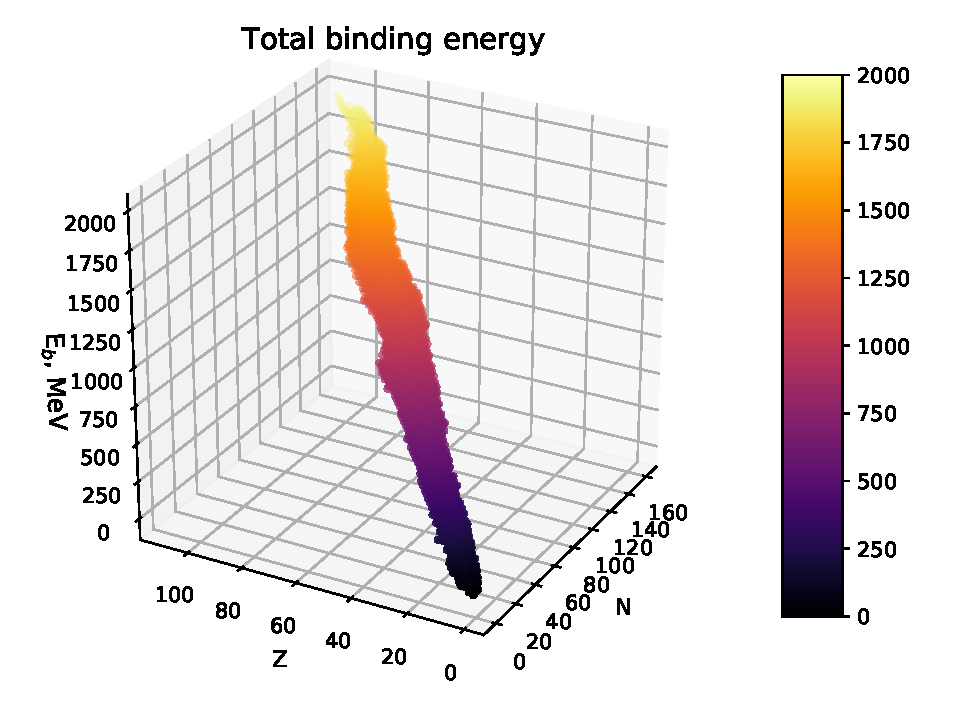
\includegraphics[width=.49\textwidth]{Figures/Total_binding_eng.pdf}
    \caption{Total binding energy expressed in MeV for the AME2016 atomic mass evaluation \cite{ame16}.}
    \label{fig: total binding energy}
\end{figure}

\begin{figure}[!htb]
    \centering
    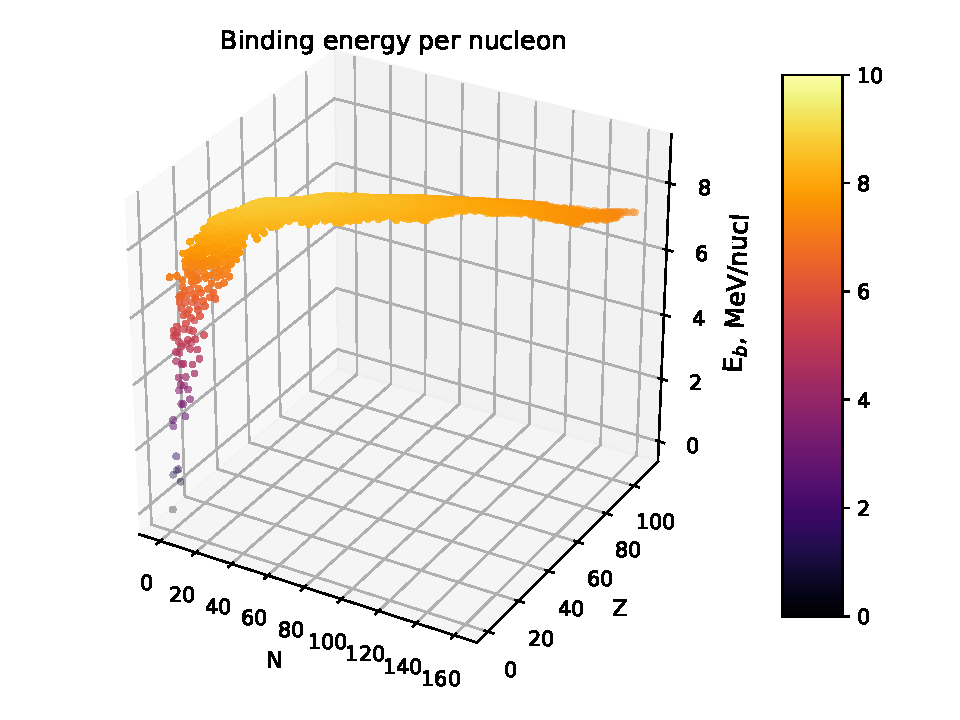
\includegraphics[width=.49\textwidth]{Figures/Binding_eng.pdf}
    \caption{Binding energy per nucleon expressed in MeV/nucleon for the AME2016 atomic mass evaluation \cite{ame16}.}
    \label{fig: binding energy}
\end{figure}

\subsection{The Duflo-Zucker Mass Model}
\label{sec: DZ}
Even though the Liquid Drop model is very useful for explaining some general features of the nucleus, it fails to explain the so-called shell effects observed in experiments. These shell effects explain how some nuclei are more tightly bound than others, due to having certain (so called magic) numbers of protons and/or neutrons, corresponding to ``full nuclear shells'' (for further details see \cite{krane}).

To include these effects, a more complex mass model can be used, namely the Duflo-Zucker Mass Model (DZ) \cite{dz}. This macroscopic model is based on the LD model and includes shell effects, and can be expressed as
\begin{equation}
E_b = \langle H_{m}\rangle - E_C - E_{\mathrm{sym}} + E_P , 
\end{equation}
where $\langle H_{m}\rangle$ is the Hamiltonian including shell effects, and $E_C$, $E_{\mathrm{sym}}$ and $E_P$ is the microscopic Coulomb, symmetry and pairing energies respectively. The version of the DZ model used in the articles we use for comparisons in this work, is the DZ10 model. This model has in total 10 terms. There is also another more complex full DZ model, with a total of 33 terms.

\subsection{The Hartree-Fock-Bogoliubov Method}
\label{sec: HFB}
Another theoretical approach of calculating the nuclear masses and binding energies is based on the Hartree-Fock-Bogoliubov method (HFB) \cite{goriely}, which is a theoretical framework for calculating the two-body interactions between a system of fermions.

It is based upon calculating the anti-symmetric two-body matrix elements in the Hamiltonian, and from this obtaining the energy eigenvalues. In short, this can subsequently be used to calculate nuclear masses.


\subsection{Machine Learning Methods}

Two new Machine Learning methods are introduced in this project, namely \textit{Decision Trees} and \textit{XGBoost}, and are both briefly described in the following subsections. For the remaining methods, we refer to Project  1\cite{proj1_1, proj1_2} and Project 2 \cite{proj2} for detailed information.


\subsubsection{Decision Trees}\label{sec: decision trees}

In the following project we introduce one more algorithm for supervised learning, namely, the decision trees. Both classification and regression problems can be solved with a decision tree, the latter is the case for this work. The principal idea behind it is to search for the descriptive features of the dataset that reproduce the target features in the best way. The former features which satisfy this criterion are also called the most informative. After finding these features, the whole dataset is split along the values of these features to achieve the maximum purity of the corresponding target feature values. This procedure, or search for the most informative features, continues until some stopping criterion is satisfied \cite{Morten}. 


A decision tree is built up of nodes and leaves that contain a portion of the data. For a node in the tree, we iterate over the data, and split the data into two nodes to maximise the descriptiveness of the node that is split. The new nodes are split further, until we reach a pre-set limit. A node which is not split any further is called a leaf. The split is done by calculating the sum of the squared residuals for each iteration, the lowest sum meaning the best split. In theory we could continue like this to make a perfect model for the training data, but this would result in overfitting. We avoid overfitting in multiple ways, one is to set a limit for how large (how many observations) the leaf need in order to be split and another is having a maximum depth of the tree, which was used in this project. 

Additionally we applied a method called cost-complexity pruning to further improve our results and avoid overfitting the training data \cite{Morten}. In addition to calculating the sum of the squared residuals for the leaves, it also applies a pruning parameter, in this work expressed as $\lambda$, that gives a certain penalty depending on the total number of leaves in the tree. The function to be minimized is then expressed as \cite{Morten}:
\begin{equation}
    \sum_{m=1}^{\bar{T}}\sum_{i:x_i\in \mathcal{R}_m}(y_i-\bar{y}_{\mathcal{R}_m})^2+\lambda \bar{T},
\end{equation}
where $m$ is the index of a terminal node, $\mathcal{R}_m$ are the subsets in the predictor space the original dataset is divided into, $\bar{T}$ is the number of terminal nodes, $\bar{y}_{\mathcal{R}_m}$ are the mean responses for each subset $\mathcal{R}_m$. The parameter $\lambda$ defines the penalty or the \textquotedblleft extra price \textquotedblright the algorithm has to pay in terms of the cost function for having too many terminal nodes. Essentially what this does is that it removes some leaves, so that we avoid overfitting and improves the overall performance of our decision tree.


\subsubsection{XGBoost}\label{sec: XGBoost}

XGBoost (XGB) is a ``Scalable Tree Boosting System"  released in 2016 \cite{xgboost}. It is essentially a framework for gradient tree boosting, using a parallelizable core algorithm. In addition, XGB adds regularization in order to prevent overfitting. The core algorithm has won several Machine Learning prices and competitions since its release.

The gradient boosting technique combines weak-learners in to a strong learner by an iterative procedure. In the presented XGBoost model, the weak learners are decision trees with a maximum depth. At each iteration, a tree is created and then ``pruned". Pruning here means cutting of the excess branches with a relation between the gain, the parameters $\gamma$ and $\lambda$. Then the small tree, or weak learner, is added together with the other trees. A final output is then obtained as illustrated from

\begin{equation}
    O(\mathrm{final}) = \sum_{i=1}^N\eta \times O(x_i)
\end{equation}
with $O$ representing the output value, $x_i$ representing one weak learner and $\eta$ the learning rate.

\subsubsection{Other methods}\label{sec: Other methods}

In this section we present a brief reminder on the linear regression methods as well as the feed forward neural networks additionally applied in this project. 

The core objective of the learning procedure in a neural network as well as in the linear regression is to find a set of optimal parameters minimizing the difference between a prediction made $\tilde{\textbf{Y}}$ and a real observed (target) value \textbf{Y}. This difference is expressed in terms of the cost function. Let us consider the cost function for the regression problem, namely the sum of squared residuals, or the mean squared error:
\begin{equation}
\begin{split}
      C(\textbf{Y},\tilde{\textbf{Y}})=&\frac{1}{n}(\textbf{Y}-\tilde{\textbf{Y}})^T(\textbf{Y}-\tilde{\textbf{Y}}),
\end{split}
\end{equation}

Further, we write the predicted value  $\tilde{\textbf{Y}}$ explicitly as $\tilde{\textbf{Y}}=\textbf{X}\boldsymbol{\beta}$ in terms of the design matrix $\textbf{X}$ built from the predictor variables and the regression parameter $\boldsymbol{\beta}$ \cite{Morten}. The Ordinary Least Squares (OLS) method studied in \cite{proj1_1,proj1_2} exploits an analytical expression for the optimal regression parameter $\boldsymbol{\beta}$, minimizing the cost function.  Parameter $\boldsymbol{\beta}^{\mathrm{OLS}}$ is given by the following equation:

\begin{equation}
    \boldsymbol{\beta}^{\mathrm{OLS}} = (\mathbf{X}^T \mathbf{X})^{-1} \mathbf{X}^T \mathbf{Y}.
    \label{eq:beta-ols}
\end{equation}

Here the matrix $\mathbf{X}^T\mathbf{X}$ is inverted, which can be a heavy computational operation or can not be performed if $\mathbf{X}^T\mathbf{X}$ is a singular matrix. This is effectively accounted for in ridge and LASSO regression methods, adding the penalized 2-norm and 1-norm of the regression parameter  \boldsymbol{\beta} respectively (see \cite{proj1_1,proj1_2}).

The feed forward neural network exploits a similar mechanism of minimizing the cost function. This is performed by forming the matrices of weights and biases and updating them in a forward pass through the network. This process is performed until all epochs are accomplished of a certain accuracy is reached. For the deeper insight into the FFNN we refer to the second Project \cite{proj2}. As for a typical regression problem, a simple linear output activation function will be used in this project.

Finally, one of the methods the results will be compared with is the Bayesian neural network, exploited in \cite{utama2017}. Formally, one can define it as a stochastic NN trained using Bayesian inference. \cite{Bayesian}. A stochastic NN performs a so-called ensemble learning, where a set of models is trained instead of one and their predictions are accumulated. The models are simulated with their associated probability distributions. Finally, according the Bayesian inference, the model is trained by updating the probability of the hypothesis as more information regarding it becomes available. The Bayesian NN is included only in form of the results from \cite{utama2017} to be compared with.

%-----------------------------------------------------------
\section{Code} \label{sec: Code}
All programs used in this project can be found at the GitHub address in Appendix \ref{Appendix: github}.

This project was structured in an object-oriented way, by analogy with the Project 2 \cite{proj2}. As it was previously shown in \cite{proj2}, this way of organizing the program provides an effective interaction between the different objects and methods and can be easily adapted to different tasks and datasets. The \texttt{src} directory contains all files with classes for the different families of methods. Most of the files were adopted from \cite{proj2} and modified correspondingly for the work with the new dataset. For example, the \texttt{resampling\_methods.py} file contains the description of the functions organizing a model performing either a fit coupled with the k-fold cross validation or without it. Whilst the fit itself is performed by setting an object of the class  \texttt{Fitting}, contained in \texttt{regression\_methods.py} and combining, \textit{e.g.}  \texttt{OLS}, \texttt{ridge}, \texttt{logistic\_regression}, \texttt{XGB}. The \texttt{Data} class in \texttt{data\_processing.py} processes the mass tables and splits them in the arrays of used variables, namely, the proton number $Z$, neutron number $N$, mass number $A$ and binding energies. It also constructs the design matrices, performs scaling, rescaling with the \texttt{sklearn.preprocessing.StandardScaler} functionality from Scikit-Learn  \cite{skl}. In addition, splitting into the test and training datasets is performed by a class method with \texttt{sklearn.model\_selection.train\_test\_split} functionality from \cite{skl}. 

The XGBoost method was implemented from its open source software library \cite{xgboost software}.
The Decision Tree method used for this project, was taken from the Scikit-Learn software library \cite{skl}.

Processing of the data is performed by the separate files shown together with all other code components in Fig.\ref{fig: code}. To avoid confusion, the all analysis option are kept in separate files, namely \texttt{linear\_regression\_analysis.py} (for the linear regression), \texttt{neural\_network\_analysis.py} (for the FFNN), \texttt{XGB\_analysis.py} (for XGBoost), and \texttt{decisiontree\_analysis.py} (for decision trees). In the first file a user can choose an option of running with or without k-fold cross-validation, while the regression option is defined by switching between  OLS, ridge and LASSO. The program performs the grid search over different polynomial degrees and regularization parameters. As it was shown in the Project 2, the self-written FFNN demonstrated exceptionally good performance for both the regression and classification tasks, therefore, it was also used in this project. In the \texttt{neural\_network\_analysis.py} file a user can choose an option for study of the scores as functions of numbers of hidden layers (for a given number of neurons per layer), number of neurons in a layers, grid search with respect to the learning rate and regularization parameter $\lambda$. Similarly, the \texttt{decisiontree\_analysis.py} performs the search for an optimal combination of $\lambda$ and depth, whilst in the  \texttt{XGB\_analysis.py} the three dimensional search in the space of the learning rate $\eta$, depth and $\lambda$ is performed. All results are written to the files which can be found in \texttt{Files}.
The \texttt{print\_and\_plot.py} script exploits these files to plot the figures presented in this project and collected in the \texttt{Figures} folder.

All of the heatmaps in Appendix \ref{sec: appendix figures} are produced with this \texttt{print\_and\_plot.py} script.

\begin{figure}[!htb]
    \centering
    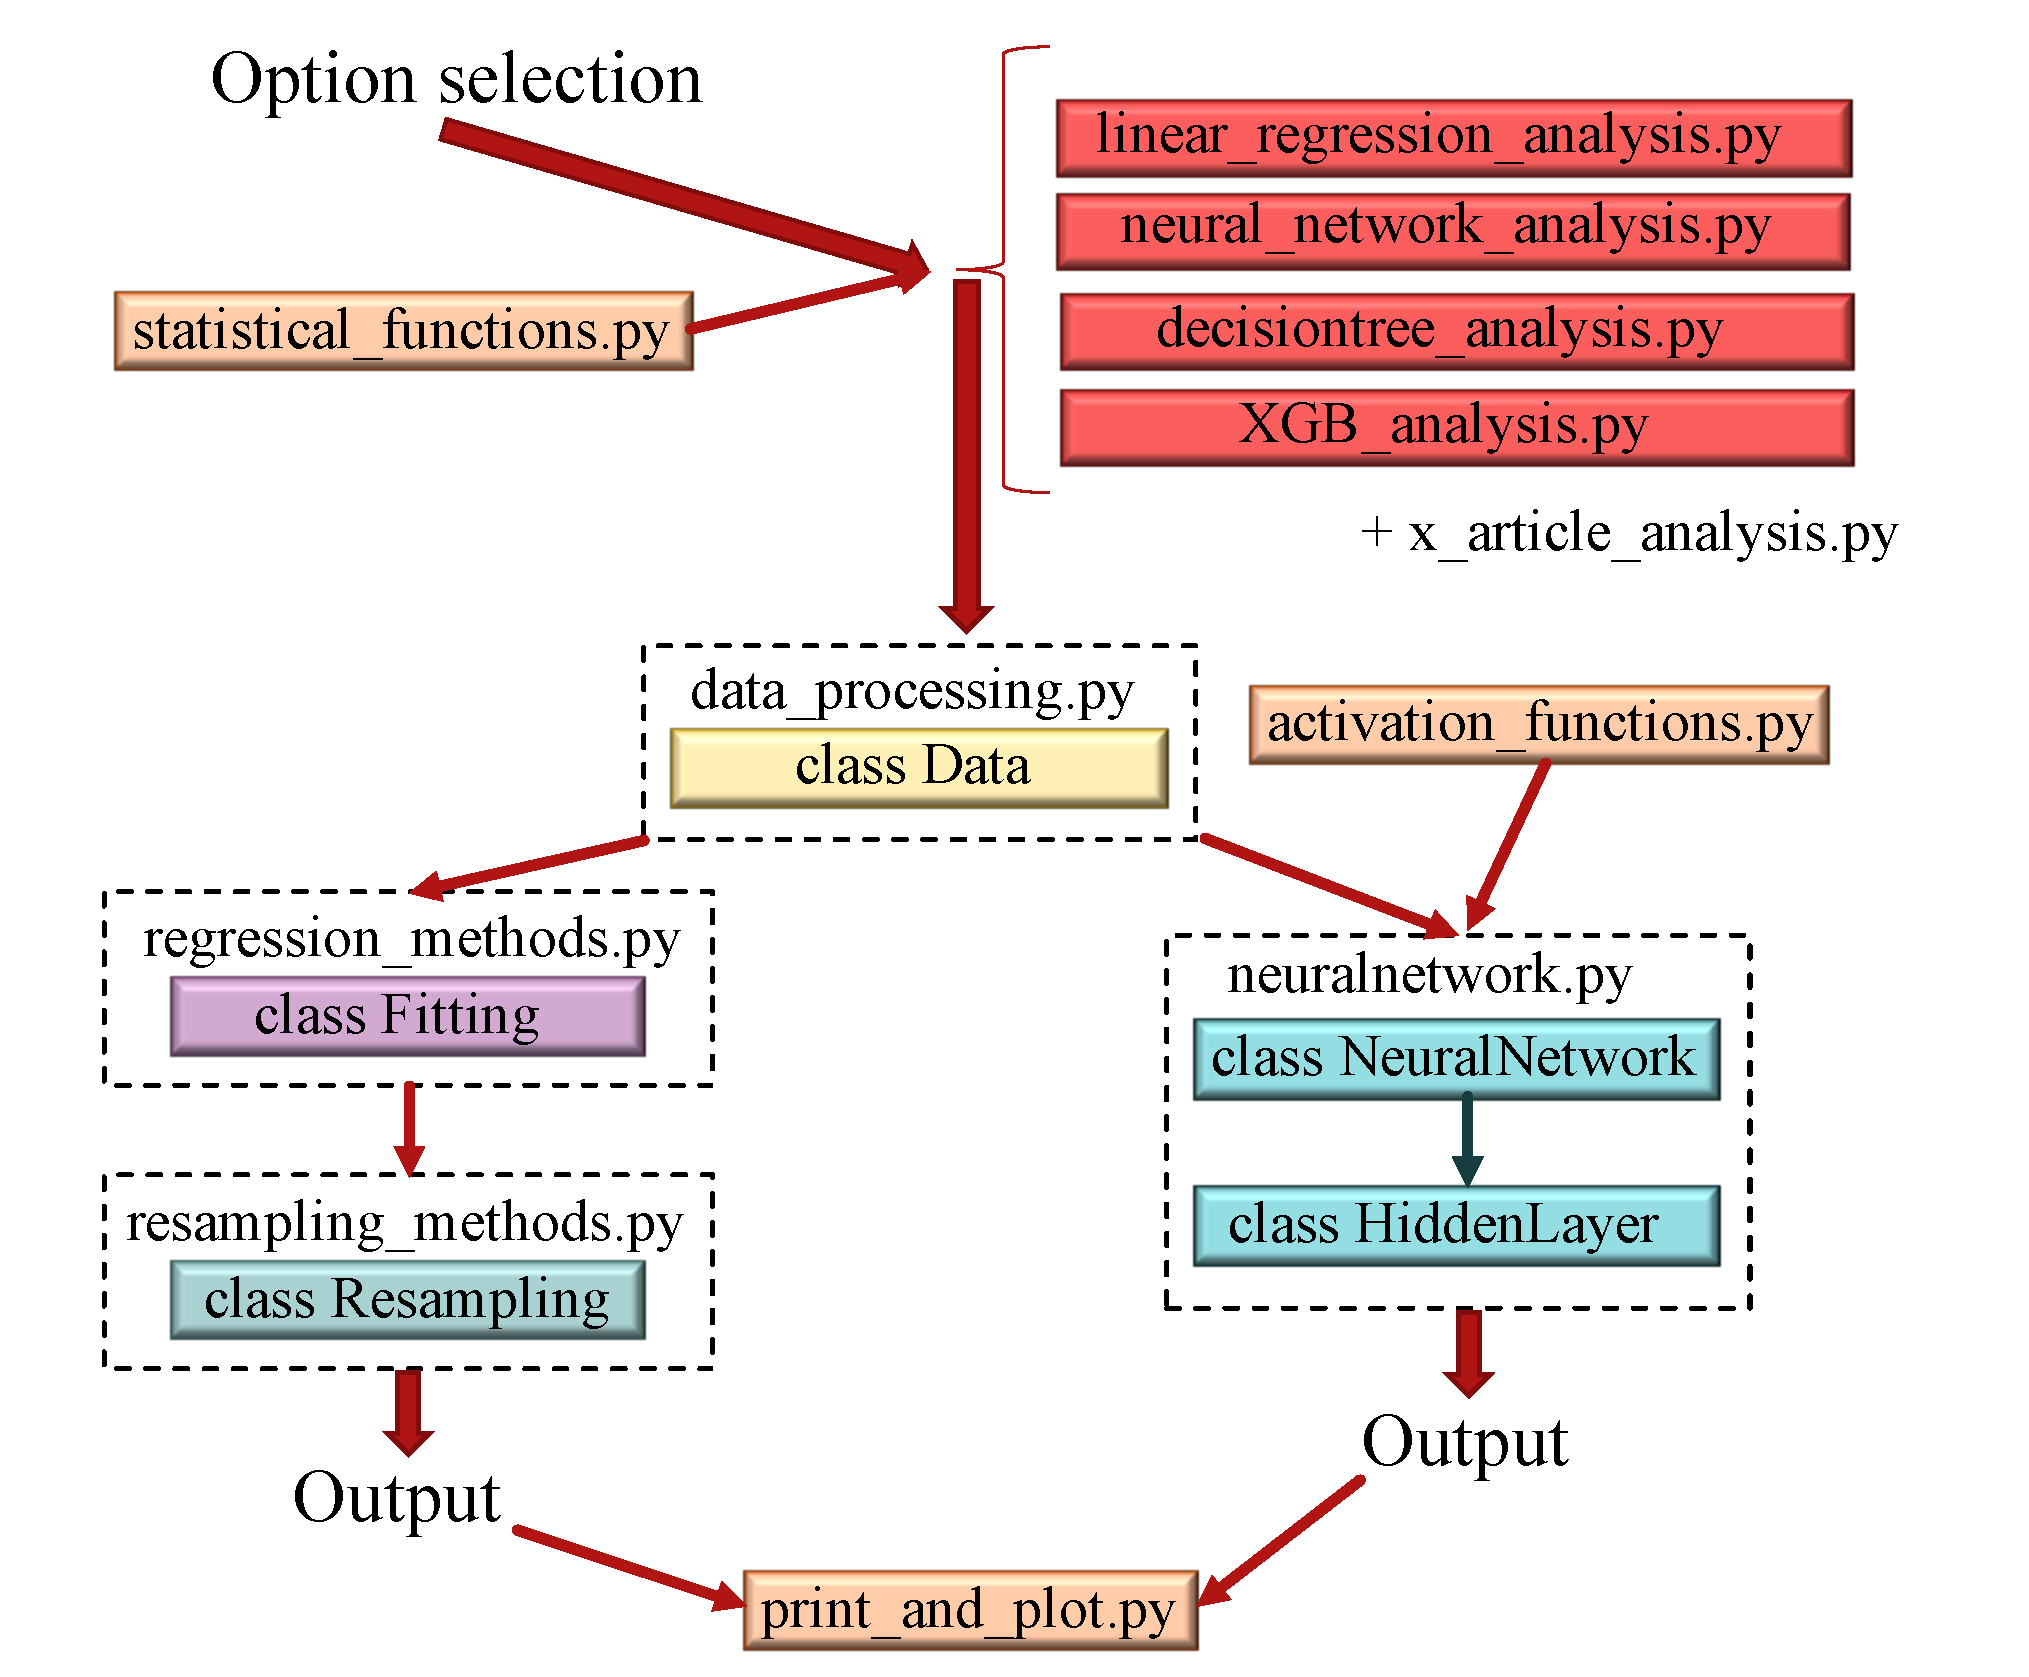
\includegraphics[width=.49\textwidth]{Figures/code.pdf}
    \caption{The principal scheme of the code used in this project.}
    \label{fig: code}
\end{figure}

 The \texttt{Data\_AME16} directory contains the data from the Atomic Mass Evaluation of 2016. Finally, the test runs showing the presented results are shown in the \texttt{project3\_testrun.ipynb} notebook.


The comparison between all the models was done with a regular train-test split (80\%-20\%), by analogy with the previous projects. However, in order to compare our results with the published values, we did a customized split of the data. The results presented in \cite{utama2017, trees in nuclear} practically exploit both from the data from the AME2016 and AME2012 database, presenting predictions for the new 46 isotopes included into AME2016. Similar was performed in this project. A model was trained and validated on the data from the AME2012 database (equal to AME2016 without the 46 new isotopes), while the test results are obtained by fitting this model on the 46 new masses. Hence the data were split twice: Firstly, the masses to be used for comparison were taken out of the main data. Secondly, the leftover data was then split into a training and a validation part in proportion 80\% to 20\%. Fig. \ref{fig: validation} illustrates how the data were split.

\begin{figure}[!htb]
    \centering
    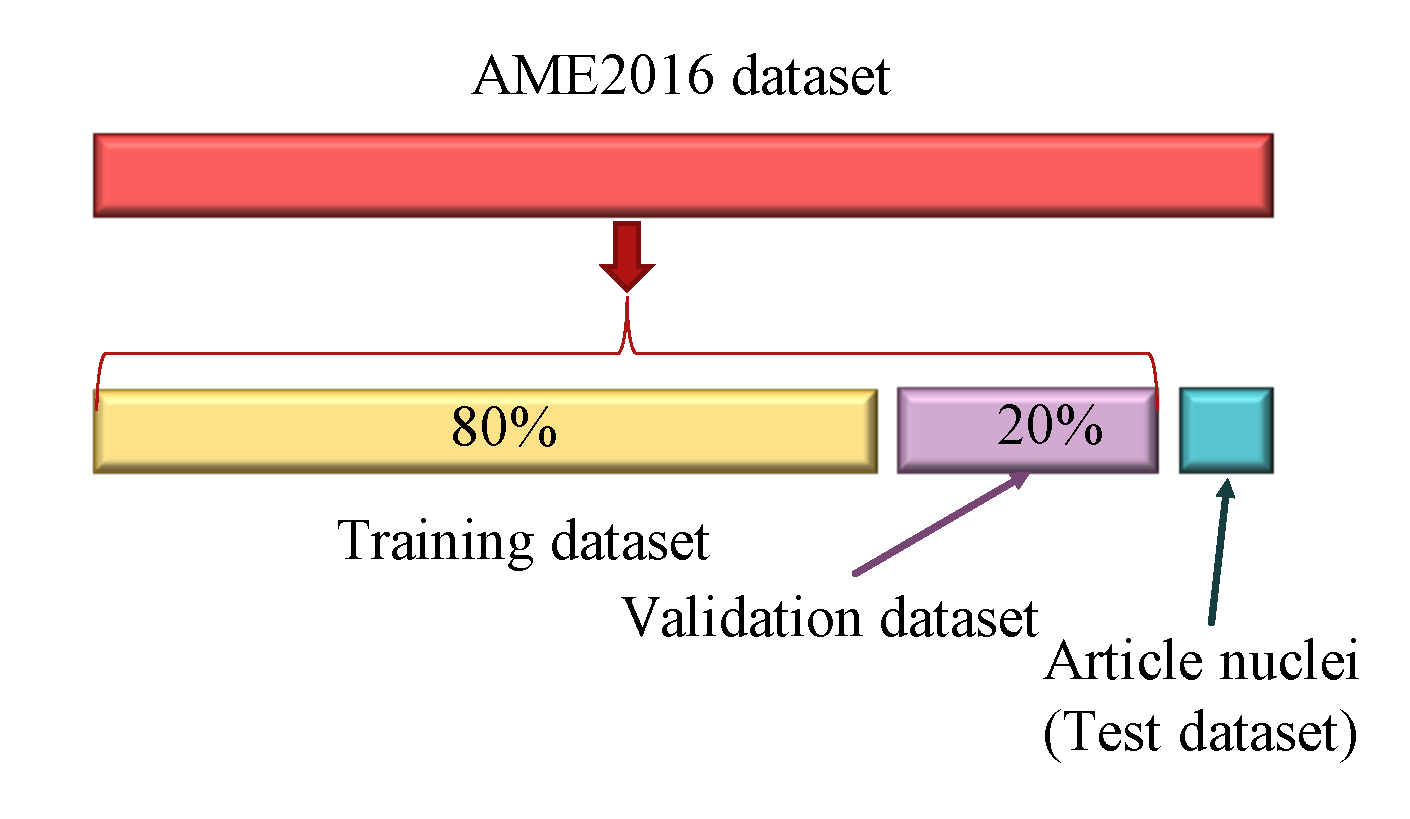
\includegraphics[width=.49\textwidth]{Figures/Validation.pdf}
    \caption{Splitting of the dataset into the training, test and validation sets.}
    \label{fig: validation}
\end{figure}



%-----------------------------------------------------------------
\section{Results}
\label{sec: Results}

Firstly, all four methods, mentioned in the previous sections, were tested for the dataset including the values of nuclear binding energies per nucleon (see Fig. \ref{fig: binding energy}). The fact that the values of binding energies can be simply presented as a 3D map with $x$-coordinates corresponding to the number of neutrons $N$ and $y$-coordinates corresponding to the number of protons $Z$ suggest the linear regression methods to be used by analogy with the Project 1 \cite{proj1_1, proj1_2}. Here, we choose to build up the design matrix for products of the polynomial degrees of $N$ and $Z$, \textit{i.e.} 1, $N\times Z$, $N^2 \times Z^2$, $N\times Z^2$, $N^2 \times Z$, ..., $Nˆp\times Z^p$. Here, $p$ is the maximum polynomial degree. As it was already mentioned, this is simply one of alternative ways to set the design matrix from the values of $N$ and $Z$. The option with the sum of values of $N^n$ and $Z^m$ was also tested, but led to particularly low scores and, therefore, was disregarded. 

All three regression methods, ordinary least squares, ridge and LASSO were applied to dataset. Table \ref{tab:MSE} contains the collection of the results for the test and training mean squared error (MSE, see \cite{proj1_1,proj1_2, proj2}) for all three methods obtained with the grid search for $p=1, 2,..., 23$ and regularization parameter $\lambda=10^{-6}, 10^{-5}, ..., 10^{0}$ for ridge and LASSO. The grid search had the principal aim of tracking the parameters $p$ and $\lambda$ yielding the minimum possible value of the test MSE. The map of the grid search can be also found in Appendix B, figures \ref{sec: appendix figures}, Fig. \ref{fig: Ridge scores} and \ref{fig: LASSO Score}. Table \ref{tab:R2} contains the corresponding test and training $R^2$ scores. All the results are presented with and without 11-fold cross-validation. As it was shown in \cite{proj1_1}, the high numbers of folds ($\approx 10$) provide good estimates of the scores. In addition, 11 folds were chosen to ensure equal division of the dataset into the batches. 


\begin{table}[!htb]
\begin{center}
\caption{Resulting MSE values for the OLS, Ridge and LASSO, both with and without 11-fold cross validation. $p_{opt}$ represents the optimal polynomial degree and $\lambda_{opt}$ shows the optimal value for the regularization parameter $\lambda$.}
\label{tab:MSE}  
\begin{tabular}{lllll}
\cline{2-5}\noalign{\smallskip}\cline{2-5}\noalign{\smallskip} 
& $p_{opt}$ & $\lambda_{opt}$ &  Train MSE & Test MSE \\ \noalign{\smallskip}\hline\noalign{\smallskip} \hline\noalign{\smallskip}
\multicolumn{1}{l|}{OLS+CV} & 17 & - & 0.0147 & 0.0241\\
\multicolumn{1}{l|}{OLS} & 19 & - & 0.0090 & 0.0457\\
\multicolumn{1}{l|}{Ridge+CV} & 19 & $10^{-1}$ & 0.0140 & 0.0230\\
\multicolumn{1}{l|}{Ridge} & 18 & $10^{-1}$ & 0.0089 & 0.0444\\
\multicolumn{1}{l|}{LASSO+CV} & 21 & $10^{-3}$ & 0.0207 & 0.0621 \\
\multicolumn{1}{l|}{LASSO} & 22 & $10^{-3}$ & 0.0162 & 0.0593\\
\noalign{\smallskip}\hline
\end{tabular}
\end{center}
\end{table}


\begin{table}[!htb]
\begin{center}
\caption{The resulting $R^2$ scores for OLS, Ridge and LASSO, both with and without cross validation. $p_{opt}$ represents the optimal polynomial degree and $\lambda_{opt}$ shows the optimal value for the regularization parameter $\lambda$.}
\label{tab:R2}  
\begin{tabular}{lllll}
\cline{2-5}\noalign{\smallskip}\cline{2-5}\noalign{\smallskip} 
& $p_{opt}$ & $\lambda_{opt}$ &  Train $R^2$ & Test $R^2$ \\ \noalign{\smallskip}\hline\noalign{\smallskip}
\hline\noalign{\smallskip}
\multicolumn{1}{l|}{OLS+CV} & 17 & - & 0.9853 & 0.9768\\
\multicolumn{1}{l|}{OLS} & 19 & - & 0.9913 & 0.9440\\
\multicolumn{1}{l|}{Ridge+CV} & 19 & $10^{-1}$ & 0.9860 & 0.9782\\
\multicolumn{1}{l|}{Ridge} & 18 & $10^{-1}$ & 0.9915 & 0.9457\\
\multicolumn{1}{l|}{LASSO+CV} & 21 & $10^{-3}$ & 0.9793 & 0.9186\\
\multicolumn{1}{l|}{LASSO} & 22 & $10^{-3}$ & 0.9844 & 0.9275\\
\noalign{\smallskip}\hline
\end{tabular}
\end{center}
\end{table}

Similar analysis was carried out with the FFNN. The same values of polynomial degrees as chosen for the linear regression ($\approx 18,19$) were found to lead to the computational overflow issues for the simplest NN architectures, low scores and unreasonably large CPU run times. By testing various potential polynomial degrees for the design matrix, it was found that $p=3$ provides the highest possible test $R^2$ for a given NN architecture, so this value was kept for this analysis. 

The next step implied optimization of the NN architecture buy selecting the number of hidden layers and neurons in the layers yielding the compromise between the run time and the high scores. In Project 2 \cite{proj2}, 50 neurons per layer were used and it was decided to take it as the starting point. The sigmoid function was used for activation of neurons in each hidden layer. Fig. \ref{fig: layers}  demonstrates how the test and training MSE changes for a NN with 50 neurons per layer with the increasing number of layers. It can be seen that increasing the number of layers leads to an overall decrease of both the test and training MSE. However, the noisy behavior at numbers of layers larger than 5 imply that the performance of the NN can not be improved dramatically simply by adding new layers. On the contrary, this will lead to the fast increase of the run time. It can be seen that already at 4 layers one can achieve the same test and training MSE value that is held in average for higher numbers of hidden layers. This number was chosen for the further analysis.

\begin{figure}[!htb]
    \centering
    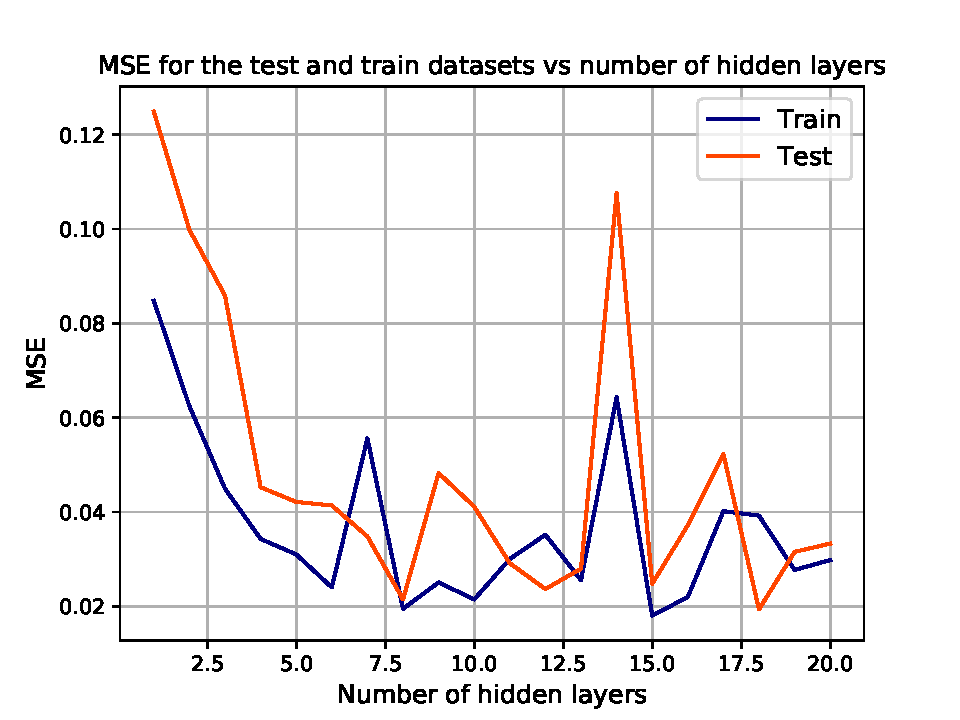
\includegraphics[width=.49\textwidth]{Figures/NN_layers.pdf}
    \caption{The test and training MSE values as functions of the number of layers in the FFNN. The network has 50 neurons per layer, 1000 epochs, $\eta=0.0001$.}
    \label{fig: layers}
\end{figure}

\begin{figure}[!htb]
    \centering
    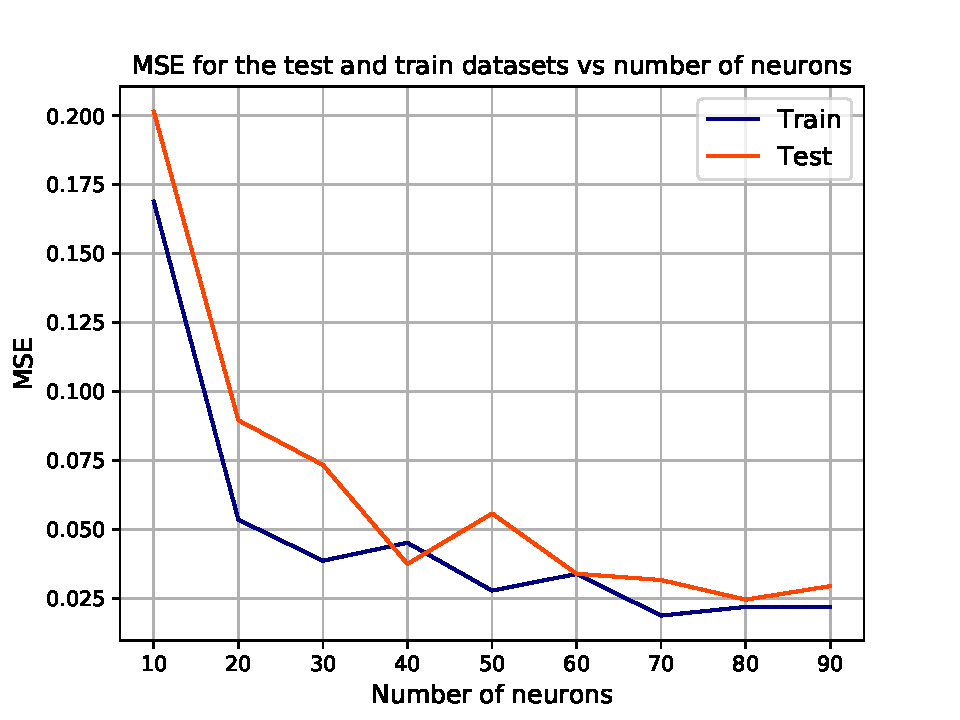
\includegraphics[width=.49\textwidth]{Figures/NN_neurons.pdf}
    \caption{The test and training  MSE values as functions of number of neurons in hidden layers in the FFNN. The network has 5 hidden layers,  1000 epochs, $\eta=0.0001$. }
    \label{fig: neurons}
\end{figure}

When the number of hidden layers is fixed, the reasonable number of neurons should be chosen to yield good performance of the NN. Fig. \ref{fig: neurons} demonstrates how the test and training MSE behave for a NN with 5 hidden layers as the number of neurons in each layer increases. In overall, a steady decrease for the MSE is observed for the increasing number of neurons. However, it also increases the computational time. Several test of different layer/neuron combinations led to a decision to use the combinations of 50, 60 and 70 layers as follows: 50 neurons in the first layer, 50 in the second, 70 in the third, 60 in the fourth. This was kept for the further analysis. 


Table \ref{tab:FFNN MSE} and \ref{tab:FFNN R2} summarize the test and training MSE and $R^2$ scores from the grid search (Fig. \ref{fig: FFNN+Sigmoid scores}), corresponding to the optimal learning rate and regularization parameter. The latter, again, yield the lowest possible test MSE. In addition to the sigmoid activation function, the tanh activation was also tested and the corresponding results can be found in Table \ref{tab:FFNN MSE} and \ref{tab:FFNN R2} and Fig. \ref{fig: FFNN+tanh scores}.



\begin{table}[!htb]
\begin{center}
\caption{The resulting test and training MSE values for the FFNN using both sigmoid and tanh as activation functions. $\eta_{opt}$ and $\lambda_{opt}$ represent the optimal learning rates and regularization values respectively. 1000 epochs are chosen.}
\label{tab:FFNN MSE}  
\begin{tabular}{lllll}
\cline{2-5}\noalign{\smallskip}\cline{2-5}\noalign{\smallskip} 
& $\eta_{opt}$ & $\lambda_{opt}$ &  Train MSE & Test MSE \\ \noalign{\smallskip}\hline\noalign{\smallskip} \hline\noalign{\smallskip}
\multicolumn{1}{l|}{FFNN+sigmoid} & 2$\cdot10^{-4}$ & $10^{-5}$ & 0.0217 & 0.0286\\
\multicolumn{1}{l|}{FFNN+tanh} & $10^{-4}$ & $10^{-1}$ & 0.0189 & 0.0777\\
\noalign{\smallskip}\hline
\end{tabular}
\end{center}
\end{table}


\begin{table}[!htb]
\begin{center}
\caption{The resulting test and training $R^2$ scores for the FFNN using both sigmoid and tanh as activation functions. $\eta_{opt}$ and $\lambda_{opt}$ represent the optimal learning rates and regulatization values respectively. 1000 epochs are used.}
\label{tab:FFNN R2}
\begin{tabular}{lllll}
\cline{2-5}\noalign{\smallskip}\cline{2-5}\noalign{\smallskip} 
& $\eta_{opt}$ & $\lambda_{opt}$ &  Train $R^2$ & Test $R^2$ \\ \noalign{\smallskip}\hline\noalign{\smallskip} \hline\noalign{\smallskip}
\multicolumn{1}{l|}{FFNN+sigmoid} & 2$\cdot10^{-4}$ & $10^{-5}$ & 0.9781 & 0.9723\\
\multicolumn{1}{l|}{FFNN+tanh} & $10^{-4}$ & $10^{-1}$ & 0.9809 & 0.9249\\
\noalign{\smallskip}\hline
\end{tabular}
\end{center}
\end{table}

The next methods to be tested are the decision trees and XGBoost. Table \ref{tab: XGB DT} demonstrates the results for decision tree and XGBoost methods. For the decision tree, the optimal results were found for maximum depth of 14 and $\lambda = 10^{-7}$.The results for the decision tree method were found in a similar grid search in the range of depths up to 14 and $\lambda=10^{-7}, 10^{-6}, ..., 10^{-1}$. Trees with the depth higher than 15 were not studied. Fig. \ref{fig: Decision Tree scores} represents the described grid search.

For XGBoost the trend for overfitting was visible at more shallow depths compared to the decision tree, as expected. A 3-dimensional grid search was used to obtain the XGBoost results, looping over different learning rates, maximum depths and $\lambda$ values. The learning rate for XGBoost was tested for values in the range $0-1$, and proved to give the best results at $\sim 0.0776$.  For $\lambda$, values from $10^{-7}-10^2$ were included in our study. The corresponding grid search is shown in Fig. \ref{fig: XGBoost scores}.


\begin{table}[!htb]
\begin{center}
\caption{ The XGBoost results are acquired with a learning rate $\eta \approx 0.0776$. $d_{opt}$ represents the optimal depth of the trees and $\lambda_{opt}$ the optimal regularization parameter.}
\label{tab: XGB DT}
\begin{tabular}{lll}
\hline\noalign{\smallskip}
\hline\noalign{\smallskip}
Parameter & Decision Tree & XGBoost \\
\hline\noalign{\smallskip}
\hline\noalign{\smallskip}
 \multicolumn{1}{l|}{$d_{opt}$} & 14 & 8 \\
 \multicolumn{1}{l|}{$\lambda_{opt}$} & $10^{-7}$ & $10^{-6}$ \\\noalign{\smallskip}\hline\noalign{\smallskip}
 \multicolumn{1}{l|}{MSE train} & 0.0038 & $1.51 \cdot 10^{-6}$  \\
 \multicolumn{1}{l|}{MSE test} & 0.0588 & $2.96 \cdot 10^{-5}$\\
 \noalign{\smallskip}\hline\noalign{\smallskip}
 \multicolumn{1}{l|}{$R^2$ train} & 0.9964 & 0.99999\\
 \multicolumn{1}{l|}{$R^2$ test} & 0.9281 & 0.99997
 \\\noalign{\smallskip} \hline
\end{tabular}
\end{center}
\end{table}

The final part of the project includes the comparison of the obtained scores with the published results. In order to do this, as it was already mentioned, the new 46 isotopes appearing in the mass evaluation in 2016 are treated as the new test set. The remaining set is split into the training and validation set. The dataset of binding energies per nucleon was substituted by the total binding energies and all four methods were tested once more on the new dataset. The results in Tables \ref{tab: ridge article}-\ref{tab: XGB article} are obtained to compare with the published articles, using the total binding energy as data. All values were found by a grid search over relevant parameters.

\begin{table}[!htb]
\begin{center}
\caption{Optimal values of parameters, test, training and validation scores using the ridge regression method with the total binding energies. $p_{opt}$ is the optimal polynomial degree and $\lambda_{opt}$ is the optimal regularization parameter. Shown up to the first different digit.}
\label{tab: ridge article}  
\begin{tabular}{llllll}
\cline{2-6}\noalign{\smallskip}\cline{2-6}\noalign{\smallskip} 
& $\lambda_{opt}$ & $p_{opt}$ & Train $R^2$ & Val. $R^2$ & Test $R^2$ \\ \noalign{\smallskip}\hline\noalign{\smallskip} \hline\noalign{\smallskip}
\multicolumn{1}{l|}{Ridge} & $10^{-5}$ & 16 & 0.99998 & 0.99998 & 0.99998\\
\noalign{\smallskip}\hline
\end{tabular}
\end{center}
\end{table}

\begin{table}[!htb]
\begin{center}
\caption{Optimal values of parameters, test, training and validation scores using the FFNN obtained with the total binding energies.$\eta_{opt}$ is the optimal learning rate and $\lambda_{opt}$ is the optimal regularization parameter. Shown up to the first different digit.}
\label{tab:FFNN article}  
\begin{tabular}{llllll}
\cline{2-6}\noalign{\smallskip}\cline{2-6}\noalign{\smallskip} 
& $\eta_{opt}$ & $\lambda_{opt}$ &  Train $R^2$ & Val. $R^2$ & Test $R^2$ \\ \noalign{\smallskip}\hline\noalign{\smallskip}
\hline\noalign{\smallskip}
\multicolumn{1}{l|}{FFNN+sigmoid} & 0.0004 & 0.01 & 0.9999 & 0.9999 & 0.9996\\
\multicolumn{1}{l|}{FFNN+tanh} & 0.0003 & 0.1 & 0.9991 & 0.9967 & 0.9885\\
\noalign{\smallskip}\hline
\end{tabular}
\end{center}
\end{table}


\begin{table}[!htb]
\begin{center}
\caption{Optimal values of parameters, test, training and validation scores using the decision tree method with the total binding energies. $d_{opt}$ represents the optimal depth and $\lambda_{opt}$ is the pruning parameter. Shown up to the first different digit.}
\label{tab: DT article}
\begin{tabular}{llllll}
\cline{2-6}\noalign{\smallskip}\cline{2-6}\noalign{\smallskip} 
& $\lambda_{opt}$ & $d_{opt}$ & Train $R^2$ & Val. $R^2$ & Test $R^2$ \\ \noalign{\smallskip}\hline\noalign{\smallskip} \hline\noalign{\smallskip}
\multicolumn{1}{l|}{Decision Tree} & 0.0 & 14 & 1.0000 & 0.9998 & 0.9996\\
\noalign{\smallskip}\hline
\end{tabular}
\end{center}
\end{table}


\begin{table}[!htb]
\begin{center}
\caption{Optimal values of parameters, test, training and validation scores using the XGBoost method with the total binding energies. $\eta_{opt}$ represents the optimal learning rate, $d$ represents the depth and $\lambda_{opt}$ is the optimal regularization parameter. Shown up to the first different digit.}
\label{tab: XGB article}  
\begin{tabular}{lllllll}
\cline{2-7}\noalign{\smallskip}\cline{2-7}\noalign{\smallskip} 
& $\eta_{opt}$ & $\lambda_{opt}$ & $d_{opt}$ & Train $R^2$ & Val. $R^2$ & Test $R^2$\\ \noalign{\smallskip}\hline\noalign{\smallskip} \hline\noalign{\smallskip}
\multicolumn{1}{l|}{XGB} & 0.102 & 0.1 & 8 & 0.99999 & 0.99996 & 0.99982\\
\noalign{\smallskip}\hline
\end{tabular}
\end{center}
\end{table}




In Table \ref{tab:comparison}, all obtained results are compared to those from Ref. \cite{utama2017} and \cite{trees in nuclear}, including theoretical models and Bayesian neural networks. In order to unify the comparison, the MSEs obtained were modified into the root-mean-square standard deviation (STD).


\section{Discussion of the results}
\label{sec: Discussion}

\begin{table}[!htb]
\begin{center}
\caption{The $\sigma_{\mathrm{rms}}$ (STD) values obtained in this study compared with the theoretical values and findings in the Utama \cite{utama2017} and Carnini \cite{trees in nuclear} articles. LD, DZ and HFB-19 are theoretical models presented in the articles (see Sec. \ref{sec: LD}, Sec. \ref{sec: DZ}, Sec. \ref{sec: HFB}), and added here for comparison. BNN denotes the Bayesian neural network (see Sec. \ref{sec: Other methods}). All quantities are given in MeV.}
\label{tab:comparison}  
\begin{tabular}{ll}
\cline{2-2}\noalign{\smallskip}\cline{2-2}\noalign{\smallskip} 
& $\sigma_{\mathrm{rms}}$ [MeV] \\ \noalign{\smallskip}\hline\noalign{\smallskip}
\hline\noalign{\smallskip}
\multicolumn{1}{l|}{HFB-19 \cite{utama2017}} & 1.093 \\
\multicolumn{1}{l|}{DZ \cite{utama2017}} & 1.018 \\
\multicolumn{1}{l|}{DZ + BNN \cite{utama2017}} & 0.479 \\
\multicolumn{1}{l|}{Decision Tree + LD \cite{trees in nuclear}} & 2.070 \\
\multicolumn{1}{l|}{Decision Tree + DZ \cite{trees in nuclear}} & 0.471 \\
\multicolumn{1}{l|}{Ridge} & 1.735\\
\multicolumn{1}{l|}{FFNN + Sigmoid} & 8.329 \\
\multicolumn{1}{l|}{FFNN + tanh} & 46.174* \\
\multicolumn{1}{l|}{Decision Tree} & 8.704 \\
\multicolumn{1}{l|}{XGBoost} & 5.688 \\
\noalign{\smallskip}\hline
\end{tabular}
\end{center}
\end{table}


The first approach to fitting the binding energies per nucleon tested in this project is the OLS method. With both with and without the 11-fold cross-validation, the optimal polynomial degree yielding the minimum test MSE value is quite high, $p\approx 18$. Both the test and training MSE ($R^2$) obtained with resampling included are slightly higher (lower) than the corresponding values obtained without resampling. As it was noticed in \cite{proj1_1,proj1_2, proj2}, the former provides a more accurate estimate of the scores, for which any random deviations from the general trend are mitigated. Therefore, the scores obtained with the cross-validation and listed in Table \ref{tab:MSE} and \ref{tab:R2} provide more reliable information on the fit. Including the regularization parameter and moving to the ridge case demonstrates, again, slightly higher values of the MSE (lower values of $R^2$) for the cross-validation case. Performing the grid search allowed to find the optimal parameter $\lambda\sim10^{-1}$ yielding slightly lower training and test MSE as compared to the OLS. Similar test of the LASSO demonstrated slightly higher test and training MSE as compared to both the ridge and OLS regression methods. The true optimal value of $\lambda$ might have been missed with insufficiently fine grid search. In overall, passing through significantly small $\lambda$ values for LASSO requires especially large CPU run times, which makes this method less preferable as compared to ridge and OLS. In overall, the ridge regression method demonstrates high $R^2$ scores on both the test and training datasets (without cross-validation), $R^2_{test}\approx 0.98$ and $R^2_{test}\approx 0.99$.

The second method applied is the FFNN with the architecture described in the previous section. It was expected to outperform the linear regression with the NN, however, the scores for the test and training $R^2$ are slightly lower than those for the ridge regression ($R^2_{test}\approx 0.97$ and $R^2_{test}\approx 0.98$, see Table \ref{fig: FFNN+Sigmoid scores}). Any changes in architecture do not lead to any extensive improvements of the scores. These changes are of rather random nature (plus/minus the reported values) than systematic. Dramatic increase of the number the number of neurons in layers might improve scores insignificantly, but leads to the increase of the run time as well as proximity of the parameters to the values yielding overfitting. These results correspond to the sigmoid activation function. As ReLU and Leaky ReLU activation functions demonstrated an exception sensitivity and a high rate of falling into the computational overflow in the previous project, they were not tested here. However, the tanh activation of the hidden layers still demonstrates high training $R^2$ score comparable with that with the sigmoid. By analogy with the Project 2 \cite{proj2}, the test score is noticeably lower than for the sigmoid function. Here, again, the tanh function leads to an effective training of the NN, but fair to middling performance on the test set. 

It is interesting to note that this situation is somewhat similar to the decision trees. The training score $R^2$ is higher than that with the sigmoid and tanh, but the performance on the test set yields $R^2\approx 0.93$ only (see Table \ref{tab: XGB DT}). Further increasing of the depth might improve this score insignificantly, but also push to the area of potential overfitting. On the other hand, XGBoost results in especially high scores for both the test and training set.


If placing tested methods according to their performance, XGBoost gave the best results followed by ridge and OLS regression. The FFNN+sigmoid method also performed well, but the grid search was far more time consuming than that for the better methods. Both the decision trees and FFNN+tanh demonstrated good training, but slightly unsatisfactory performance on the test set.


Switching from the dataset for the binding energy per nucleon to the total binding energy we encounter an overall improvement of the scores for all four methods ($R^2$ test and training is higher than 0.99). In Tables \ref{tab: ridge article}-\ref{tab: XGB article}, the R2 scores for all the methods are generally better than the previous results. For all four methods the grid searches were performed and the scores for the validation set were used as an indicator for overfitting. The ridge regression method demonstrates strikingly high performance on the training, validation and, finally, the test set. For the results produced for the comparison with the, ridge regression gave the lowest test MSE and even outperformed one of the article results (decision tree +LD, see Table \ref{tab:comparison}). 

The test $R^2$ score results correspond to the $\sigma_{\mathrm{rms}}$ results in Table \ref{tab:comparison}. As one could expect, the methods with the better R2-Test scores yield a better $\sigma_{\mathrm{rms}}$ value. Noticeable are the deviation between the values in Table \ref{tab:comparison}. When the results are scaled back, the difference between the $\sigma_{\mathrm{rms}}$ results are much larger than the differences between the $R^2$-scores. Also, one can notice the results from FFNN+tanh in Table \ref{tab:comparison}. An insignificant difference in the second digit after decimal point in the test $R^2$ value for the scaled dataset is converted to a large root-mean-square deviation for the original dataset ($\approx 46$ MeV). This indicates that the FFNN+tanh still demonstrates poor performance on the test set. 

The XGBoost was expected to outperform all other methods, it gives a reasonably low STD value, but still higher than the values reported in the article and obtained with ridge. One of potential reasons for this might be missing of the optimal values of parameters while building the grid search (the grid is not fine enought). Another reason might be hidden in the way the design matrix was constructed. As it was mentioned, $N^n\times Z^m$ structure was chosen, but $N^n+ Z^m$ might potentially lead to the better results. However, it was not chosen for this project. Lower values of the STD for the article results as compared to the values obtained in this project might be related to the fact that the chosen design matrix does not account for the underlying physical phenomena. Even the simplest LD model account for more physical aspects of the binding energy than the simple treatment of the binding energy as a function of $N$ and $Z$. All results from the chosen articles are obtained with either purely theoretical models or the machine learning methods built on these models. However, for such a simple treatment of the bonding energies as chosen for this project, the STD values achieved are quite satisfactory.

\section{Conclusions} 
\label{sec: Conclusions}
In this work we have applied several different machine learning methods to analyse the nuclear binding energies, using data from the Atomic Mass Evaluation of 2016 (AME2016). We used linear regression algorithms including OLS, ridge regression and LASSO. In addition to these models we used a feed forward neural network, decision trees and XGBoost. Using these methods the optimal fits of the binding energies per nucleon were found, and it was noted that XGBoost performed the best, with the highest $R^2$ score of $0.99997$ on the test data.

Furthermore we extended our analysis to study the total binding energies, and comparing our results with previously published studies \cite{utama2017, trees in nuclear}. The ridge regression provided the best results, with a root-mean-square deviation $\sigma_{\mathrm{rms}} = 1.735$ MeV. Compared to the published results using the Duflo-Zucker model with a Bayesian neural network and a decision tree, our results were still over a factor of $3$ worse, even though ridge regression performed a lot better than our other methods on the total binding energies. This is, however, expected for the treatment of the binding energies which does not incorporate underlying physical phenomena.



\subsection{Outlooks}

Both XGBoost and decision trees have multiple parameters that could have been tuned for optimization. In this project we focused on the depth of the trees and $\lambda$, in addition to the learning rate for XGBoost, parameters we previously have studied in this course. For the first analysis, these parameters were sufficient for XGBoost to outperform the other methods. For the comparison with the article results, ridge regression provided better results than XGBoost. This could demonstrate that XGB did not perform to its full potential, which might have been avoided by optmizing more parameters. In spite of this, XGBoost did perform better than the decision tree method, showing that the results from Carnini et al. \cite{trees in nuclear} could potentially be improved.


%////////////////////////////////////////////////////////////////
\begin{thebibliography}

\bibitem{ame16}
W. J. Huang, et al. \textquotedblleft The AME2016 atomic mass evaluation.\textquotedblright Chinese Physics C, vol. 41, no. 3, p. 030002. 2017. DOI: \url{https://doi.org/10.1088/1674-1137/41/3/030003}

\bibitem{utama2017}
R. Utama and J. Piekarewicz. \textquotedblleft Validating neural-network refinements of nuclear mass models\textquotedblright,  Phys. Rev. C 97 (2017). DOI: \url{https://doi.org/10.1103/PhysRevC.97.014306}

\bibitem{trees in nuclear}
M. Carnini and A. Pastore, \textquotedblleft Trees and forests in nuclear physics.\textquotedblright Journal of Physics. G, Nuclear and Particle Physics, vol. 47, no. 8, p. 82001. 2020. DOI: \url{https://doi.org/10.1088/1361-6471/ab92e3}

\bibitem{proj1_1}
L. G. Pedersen and M. L. Markova, \textquotedblleft Analysis of the data with the linear regression methods with application of resampling techniques\textquotedblright, October 9th, 2020. URL: \url{https://github.com/linegpe/FYS-STK4155/tree/master/Project1}, accessed December 13, 2020.

\bibitem{proj1_2}
J. E. Vevik and T. Storebakken, \textquotedblleft Regression analysis and resampling techniques\textquotedblright, October 7, 2020. URL: \url{https://github.com/tellefs/ML-projects/tree/master/project1}. Accessed December 13, 2020.

\bibitem{proj2}
M. L. Markova, J. E. Vevik and T. Storebakken, \textquotedblleft Classification and Regression - From Linear and Logistic Regression to Neural Networks\textquotedblright, November 9th, 2020. URL: \url{https://github.com/tellefs/ML-projects/tree/master/project2}. Accessed December 8, 2020.

\bibitem{krane}
K. S. Krane, \textquotedblleft Introductory Nuclear Physics\textquotedblright, Wiley, 1988. ISBN: 9780471805533.

\bibitem{dz}
 J. Duflo, A. P. Zuker, \textquotedblleft Microscopic mass formulas\textquotedblright,  Phys. Rev. C 52, R23(R) (1995).

\bibitem{goriely}
S. Goriely, and  N. Chamel, J. M. Pearson. \textquotedblleft Further explorations of Skyrme-Hartree-Fock-Bogoliubov mass formulas. XII. Stiffness and stability of neutron-star matter\textquotedblright//, Phys. Rev. C 82, 035804 (2020).DOI: \url{https://link.aps.org/doi/10.1103/PhysRevC.82.035804}


\bibitem{Morten}
M. Hjorth-Jensen, "Applied Data Analysis and Machine Learning, FYS-STK4155" - lecture notes fall 2020.

\bibitem{xgboost} Tianqi Chen and Carlos Guestrin, "XGBoost: A Scalable Tree Boosting System", CoRR abs/1603.02754, 2016, \url{http://arxiv.org/abs/1603.02754}

\bibitem{Bayesian}
L. V. Jospin, W. Buntine, F. Boussaid, H. Laga, M. Bennamoun, “Hands-on Bayesian Neural Networks - a Tutorial for Deep Learning Users'', \url{arXiv:2007.06823v1 [cs.LG] 14 Jul 2020}.


\bibitem{skl}
Scikit-learn user guide and documentation, Release 0.23.2: URL: \url{https://scikit-learn.org/stable/_downloads/scikit-learn-docs.pdf}. Accessed December 8, 2020.

\bibitem{xgboost software} XGBoost Software: \url{https://xgboost.readthedocs.io/en/latest/}. Accessed December 14, 2020




\end{thebibliography}



\newpage



\appendix

\section{Link to the GitHub repository}
\label{Appendix: github}
\href{https://github.com/tellefs/ML-projects/tree/master/project3}{Link to the project repository on GitHub}.


\section{Figures}\label{sec: appendix figures}

\begin{figure}[!htb]
    \centering
    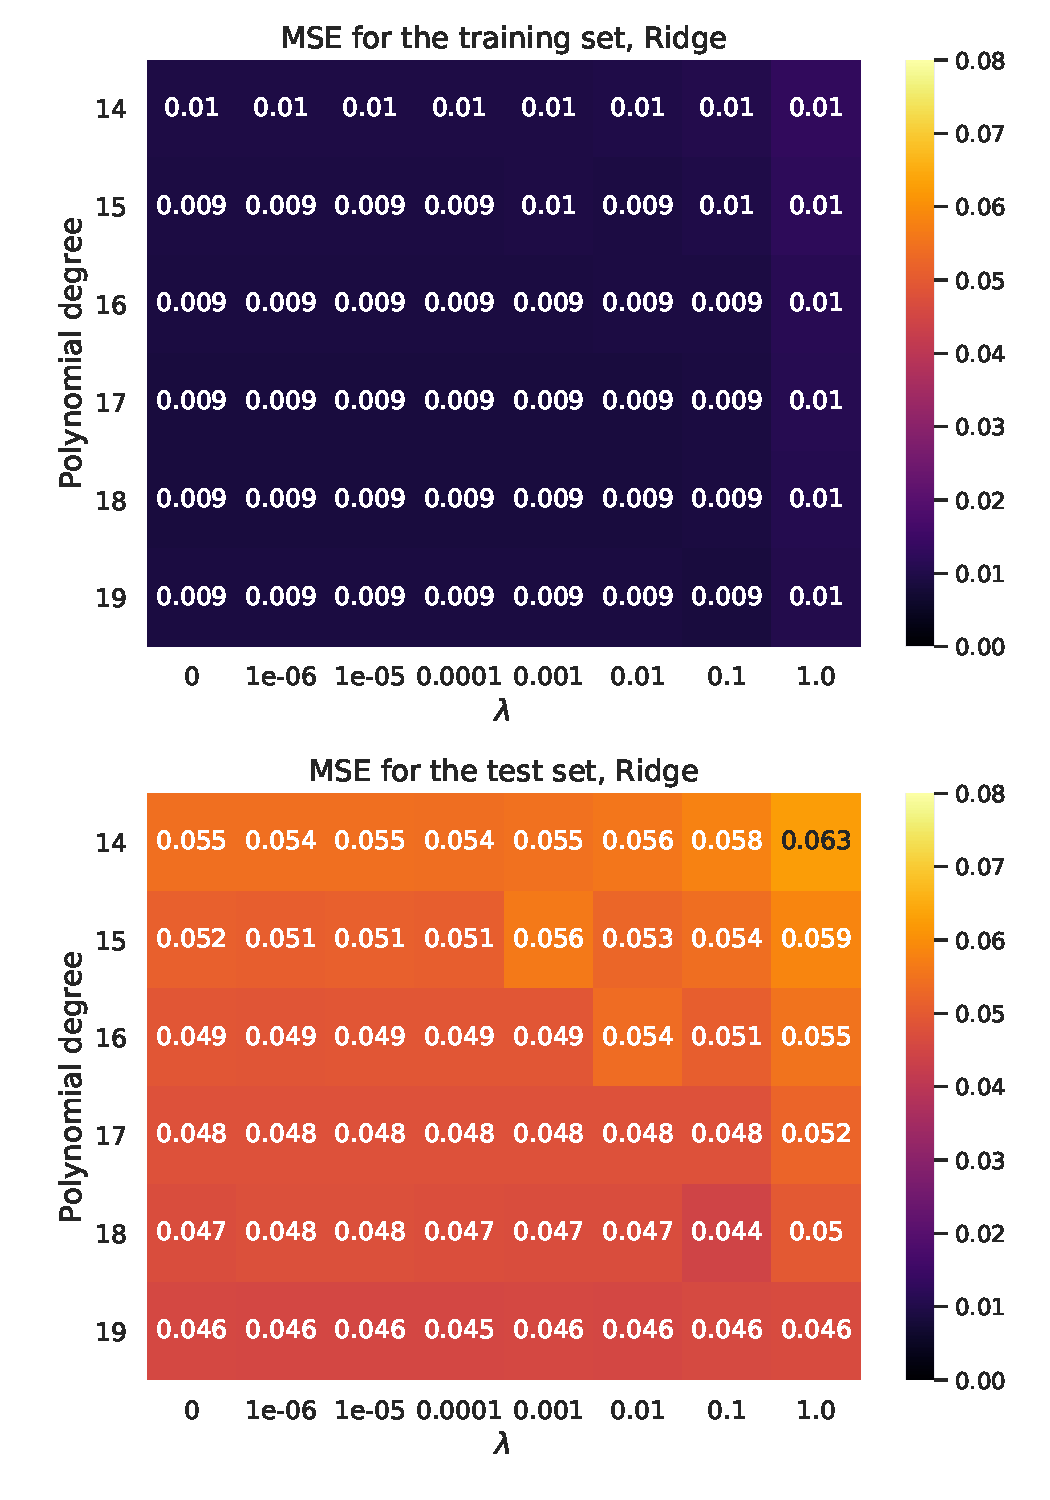
\includegraphics[width=.49\textwidth]{Figures/Ridge_MSE.pdf}
    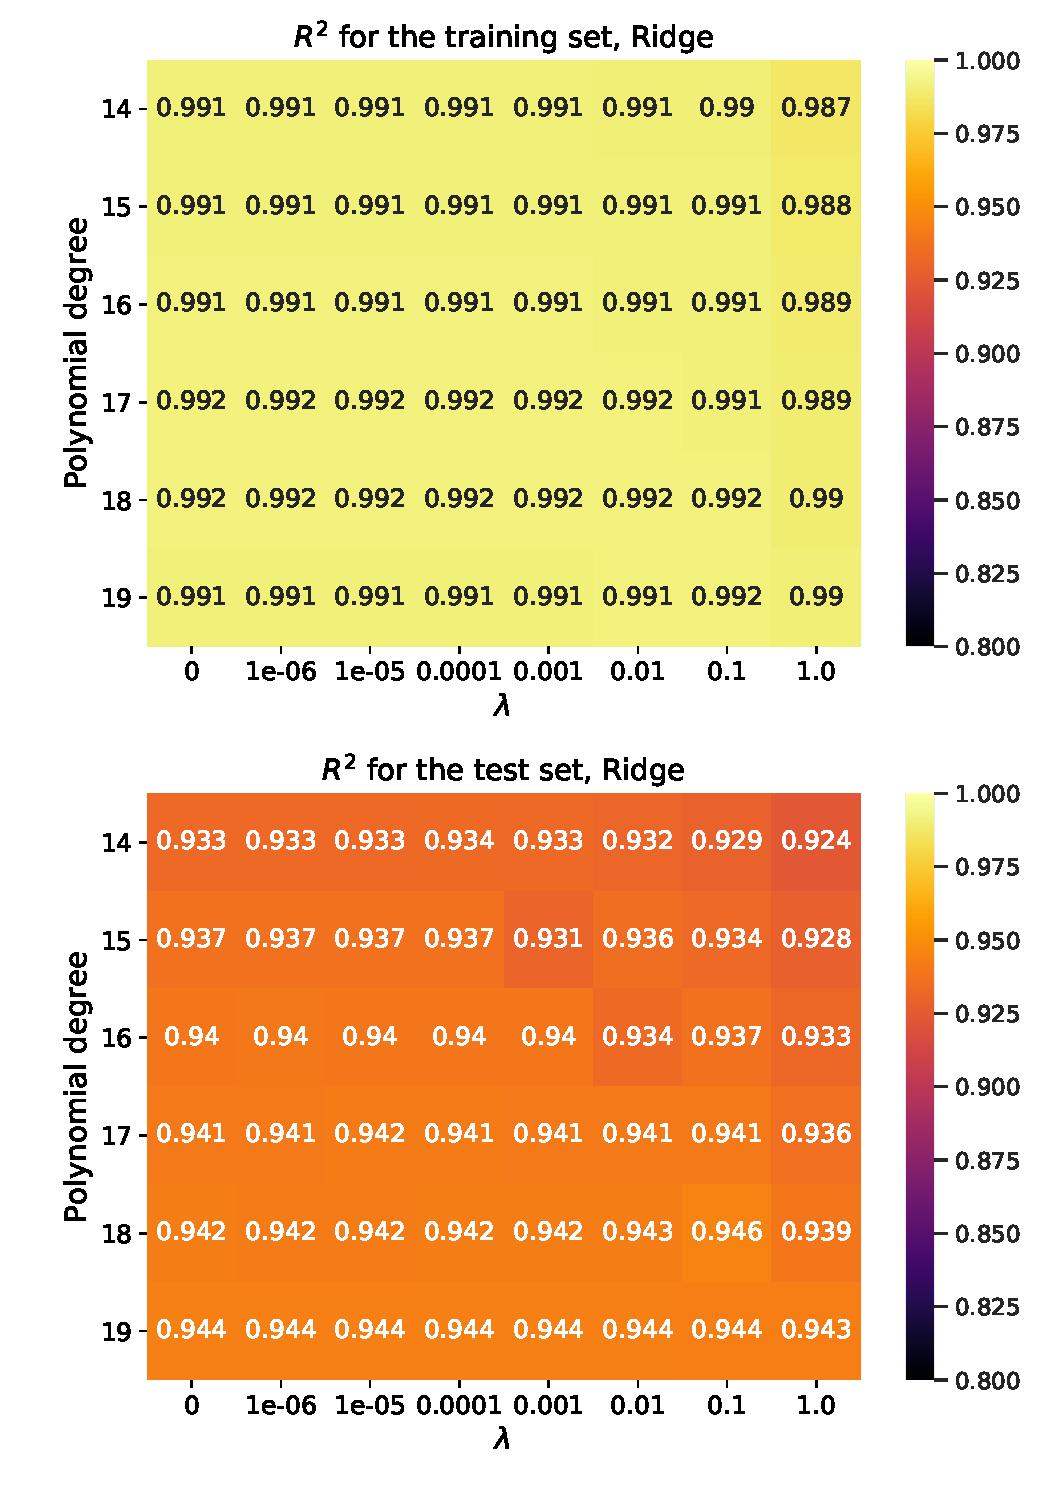
\includegraphics[width=.49\textwidth]{Figures/Ridge_R2.pdf}
    \caption{Test and training MSE (left panel) and $R^2$ scores (right panel) for the ridge regression method as functions of the polynomial degree and regularization parameter.}
    \label{fig: Ridge scores}
\end{figure}


\begin{figure}[!htb]
    \centering
    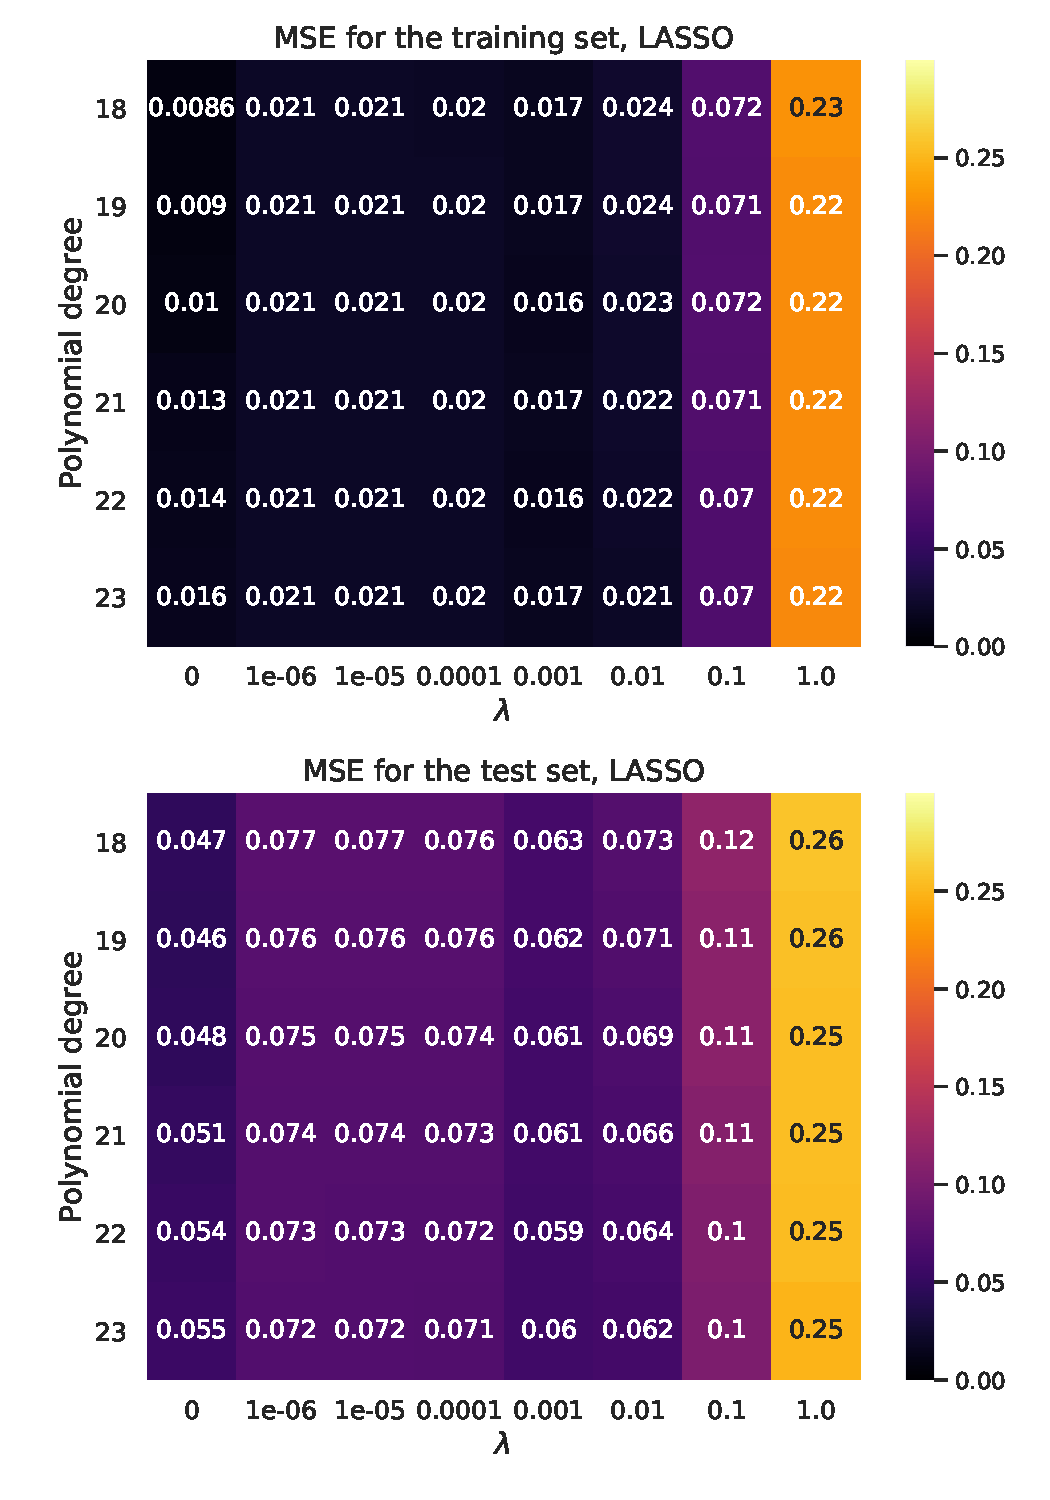
\includegraphics[width=.49\textwidth]{Figures/LASSO_MSE.pdf}
    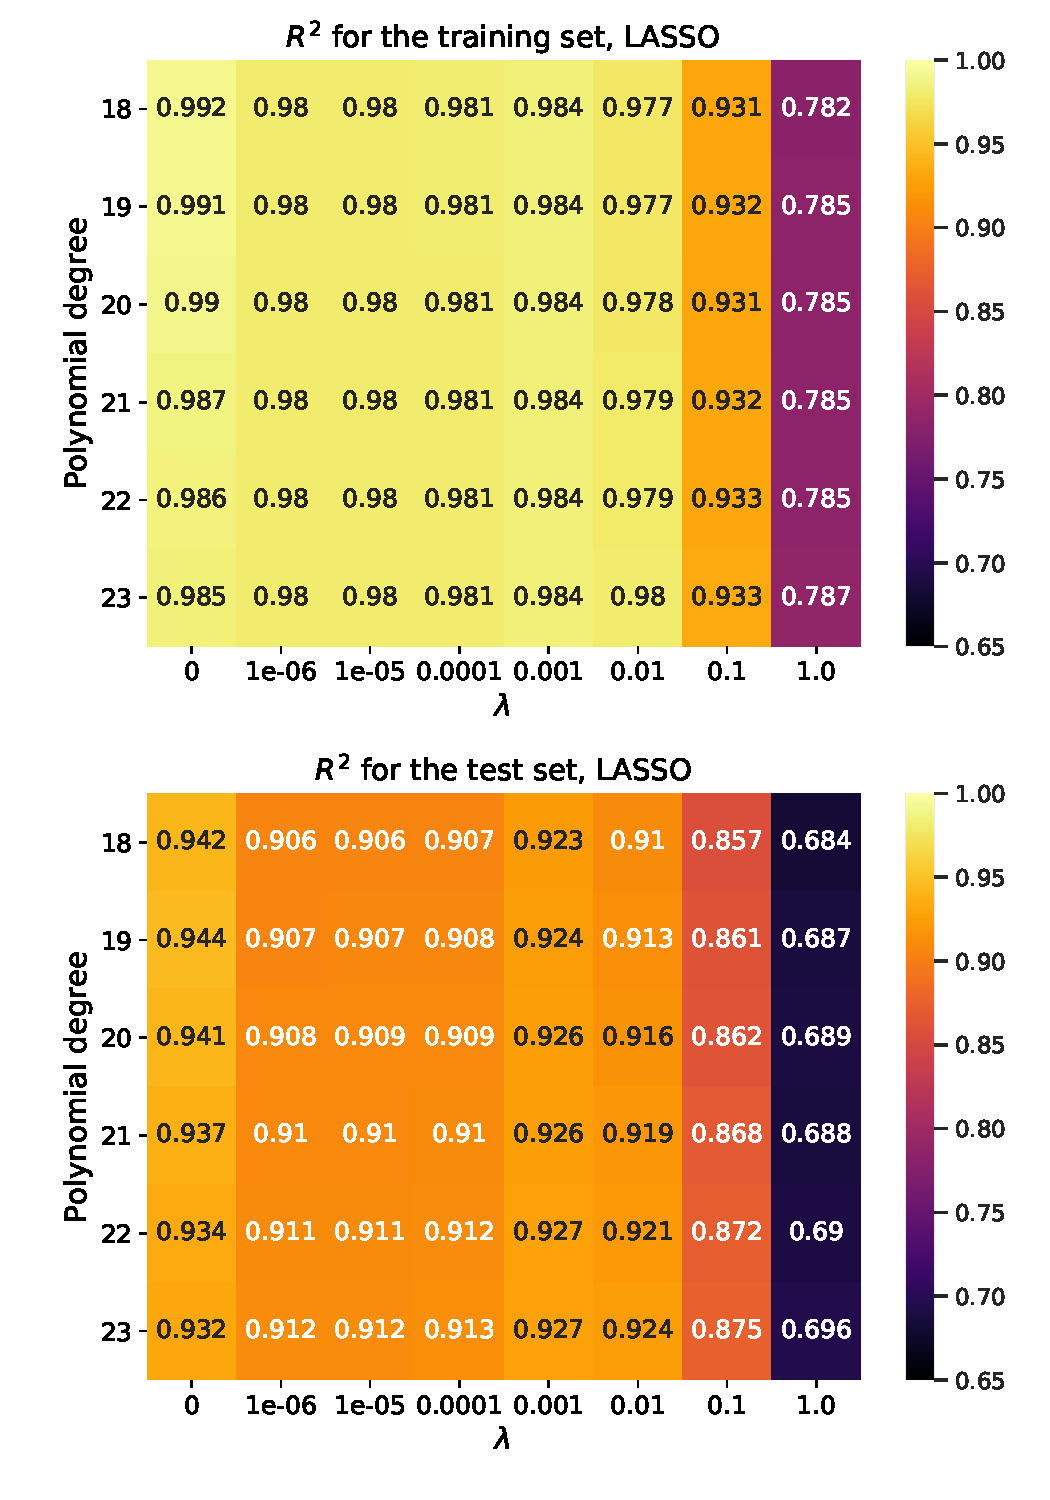
\includegraphics[width=.49\textwidth]{Figures/LASSO_R2.pdf}
    \caption{Test and training MSE (left panel) and $R^2$ scores (right panel) for the LASSO regression method as functions of the polynomial degree and regularization parameter.}
    \label{fig: LASSO Score}
\end{figure}

\begin{figure}[!htb]
    \centering
    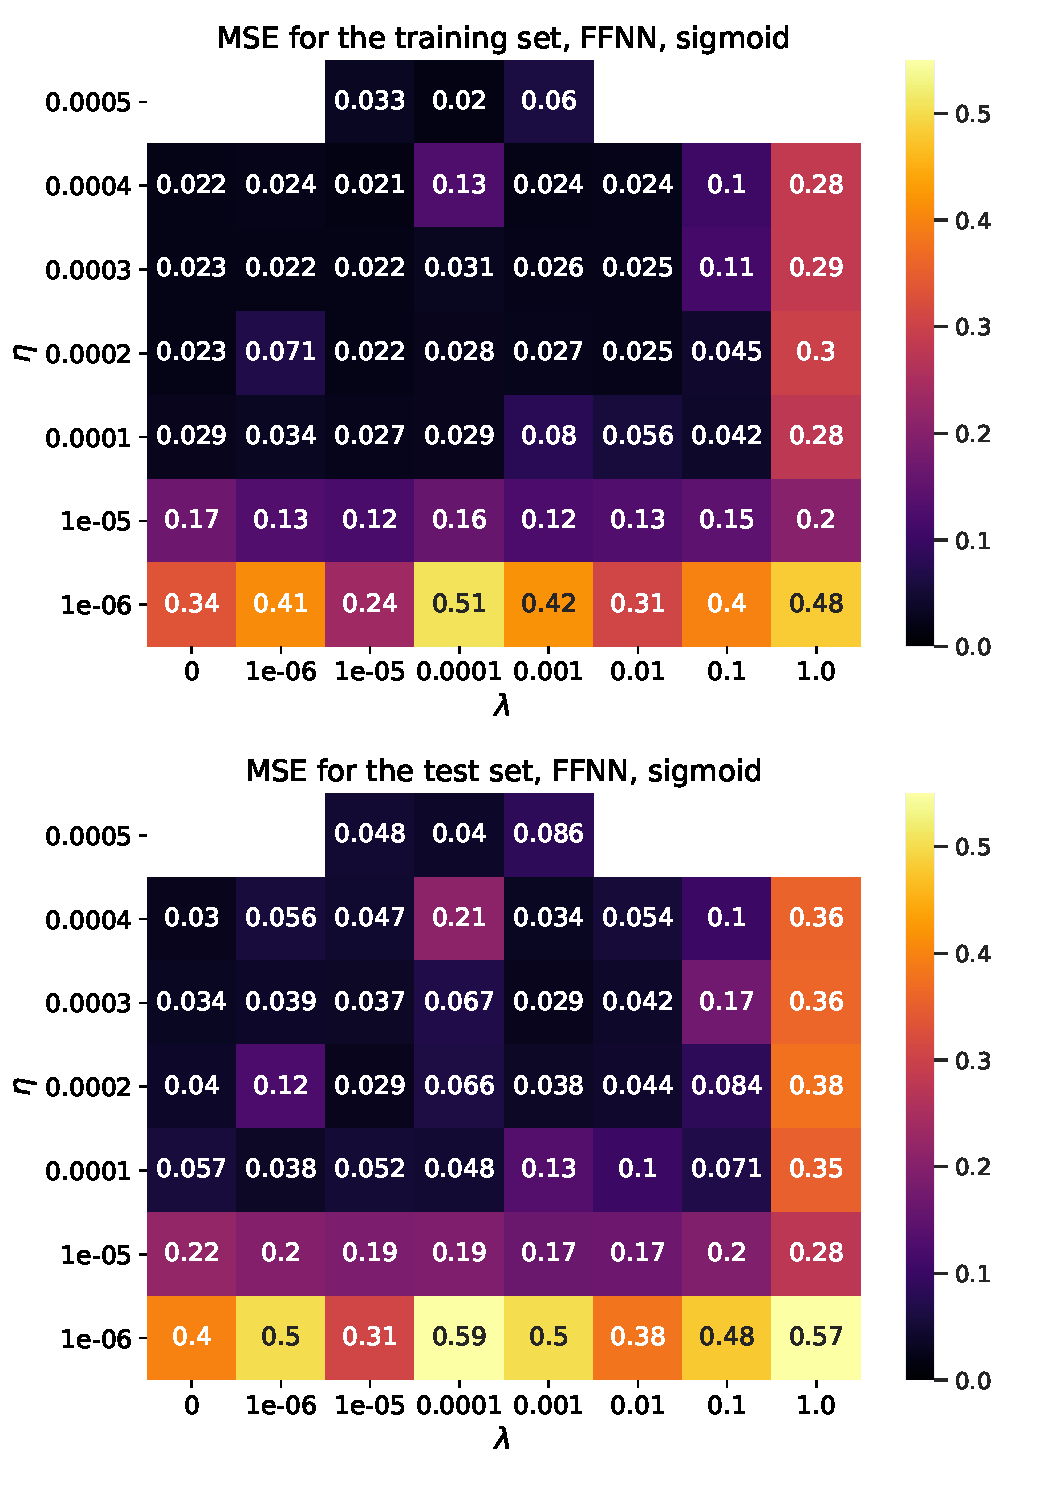
\includegraphics[width=.49\textwidth]{Figures/NN_sigmoid_MSE.pdf}
    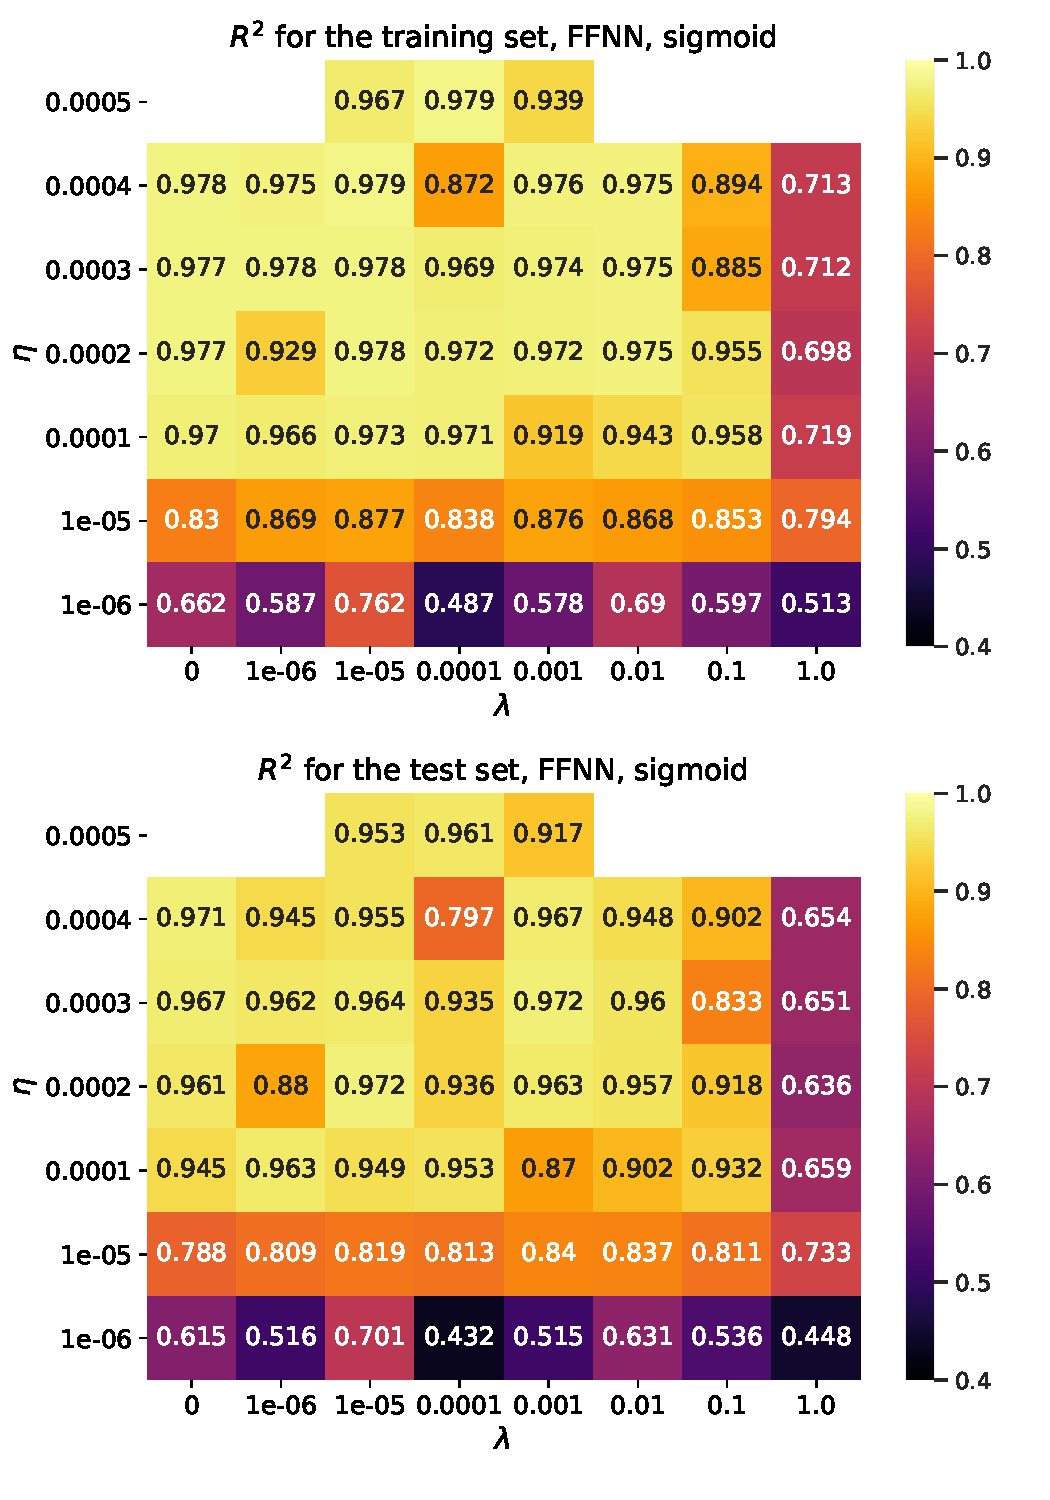
\includegraphics[width=.49\textwidth]{Figures/NN_sigmoid_R2.pdf}
    \caption{Test and training MSE (left panel) and $R^2$ scores (right panel) for the FFNN with the sigmoid activation function as functions of the learning rate and regularization parameter. 1000 epochs are used, minibatch size is 100.}
    \label{fig: FFNN+Sigmoid scores}
\end{figure}

\begin{figure}[!htb]
    \centering
    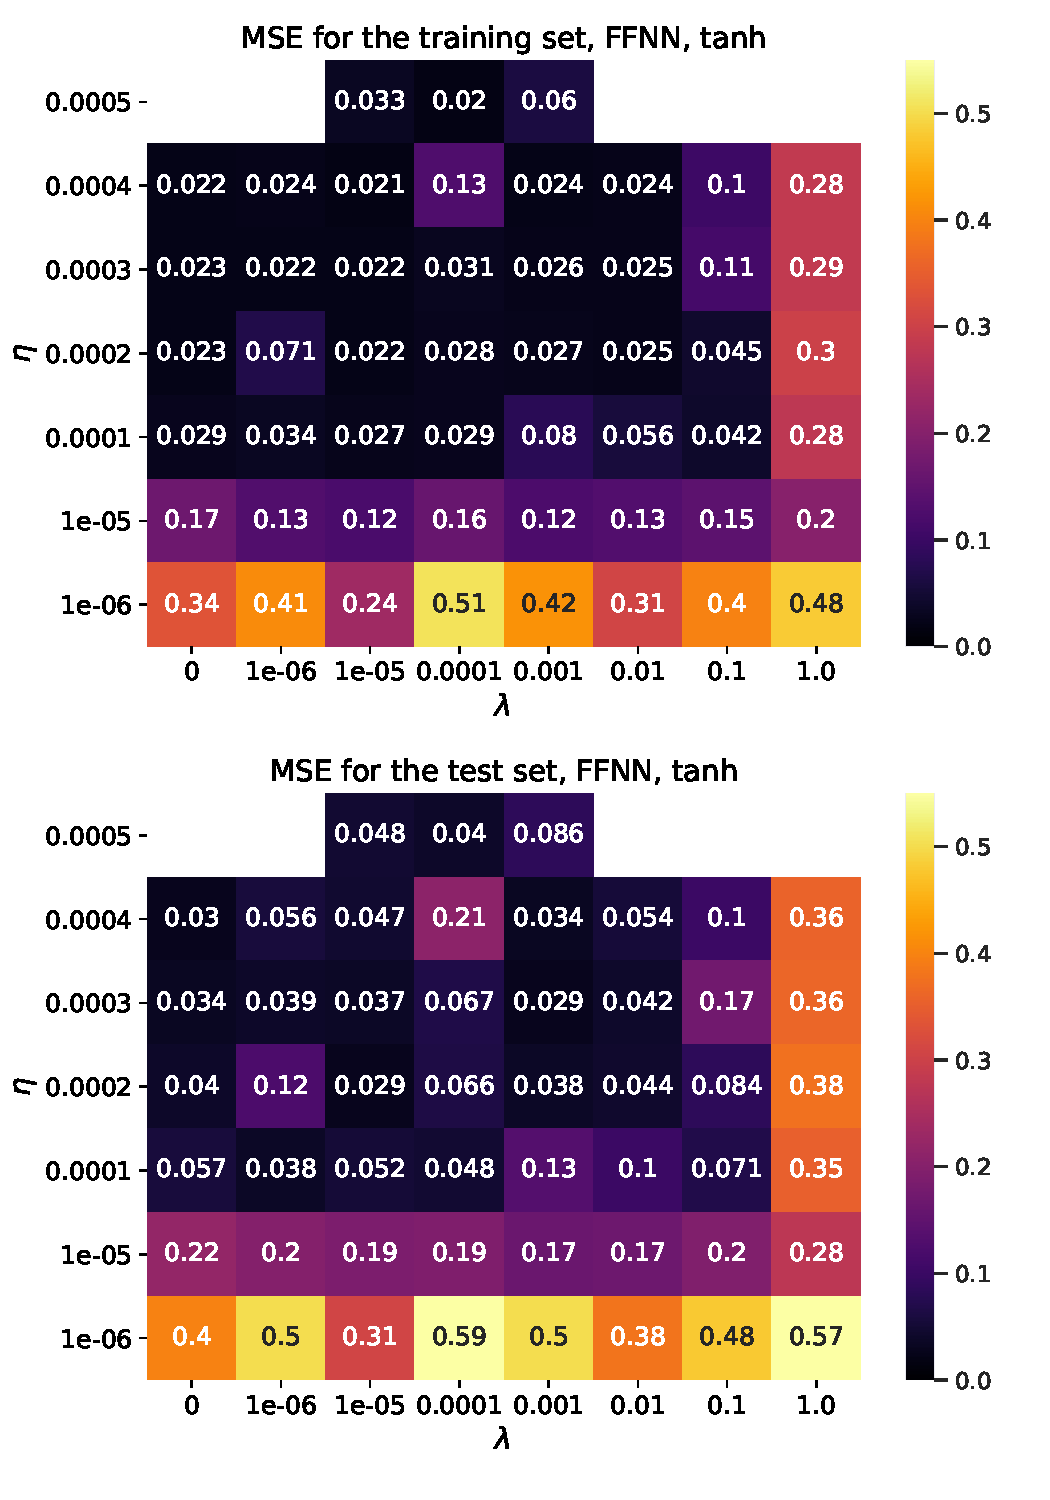
\includegraphics[width=.49\textwidth]{Figures/NN_tanh_MSE.pdf}
    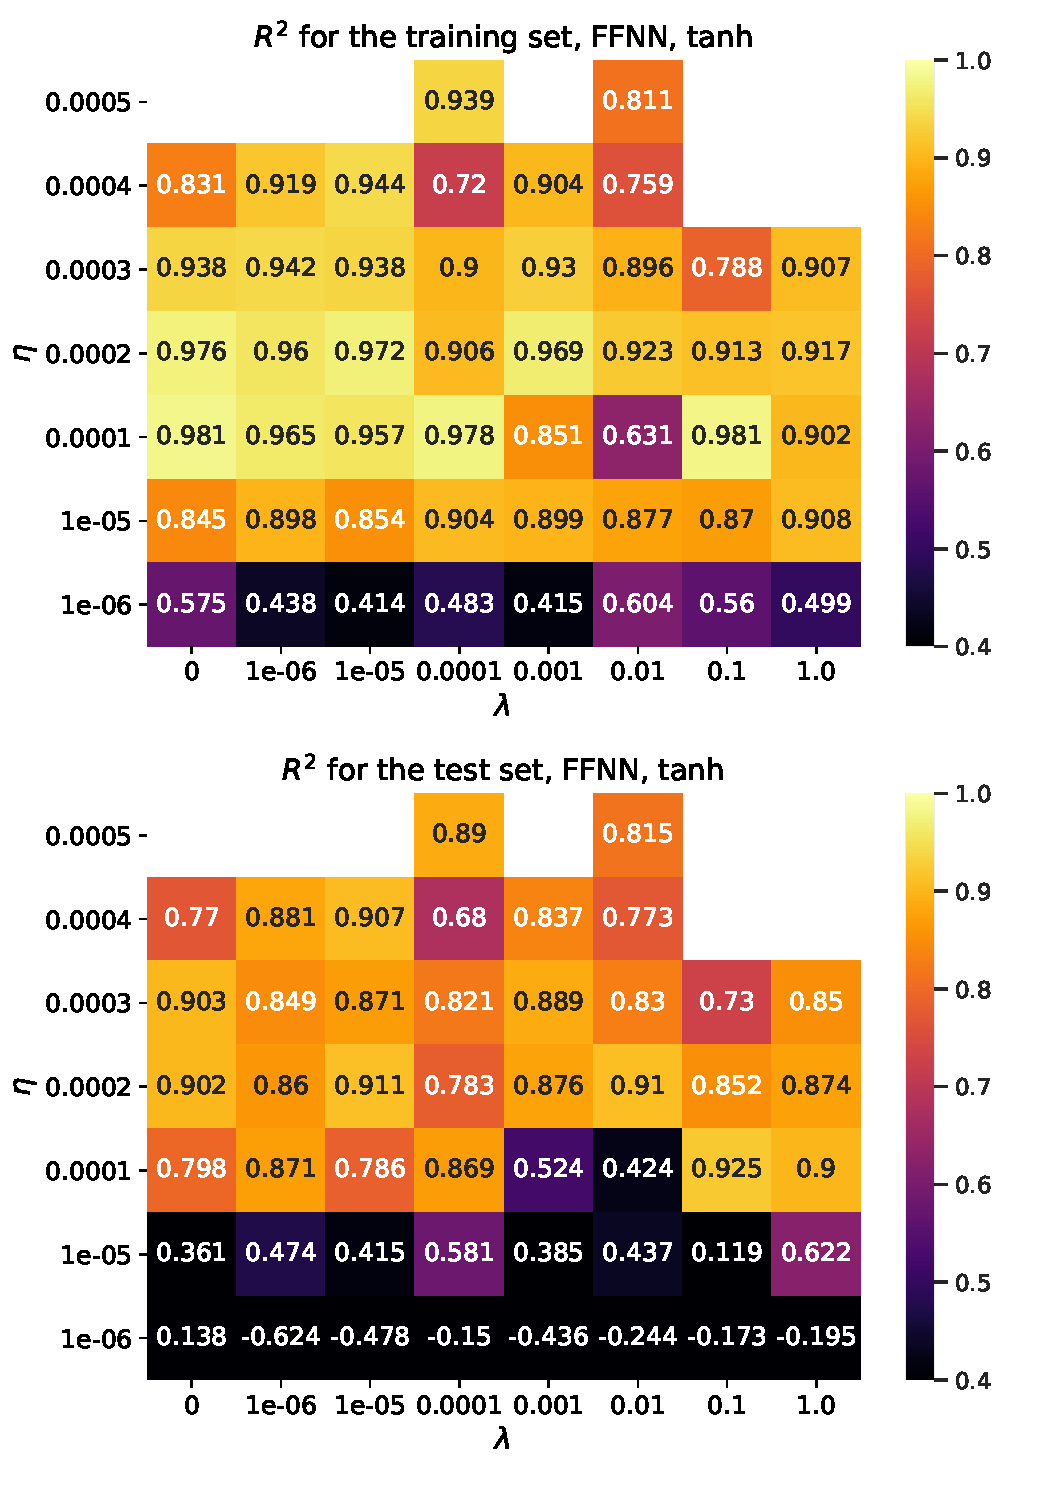
\includegraphics[width=.49\textwidth]{Figures/NN_tanh_R2.pdf}
    \caption{Test and training MSE (left panel) and $R^2$ scores (right panel) for the FFNN with the tanh activation function as functions of the learning rate and regularization parameter. 1000 epochs are used, minibatch size is 100.}
    \label{fig: FFNN+tanh scores}
\end{figure}

\begin{figure}[!htb]
    \centering
    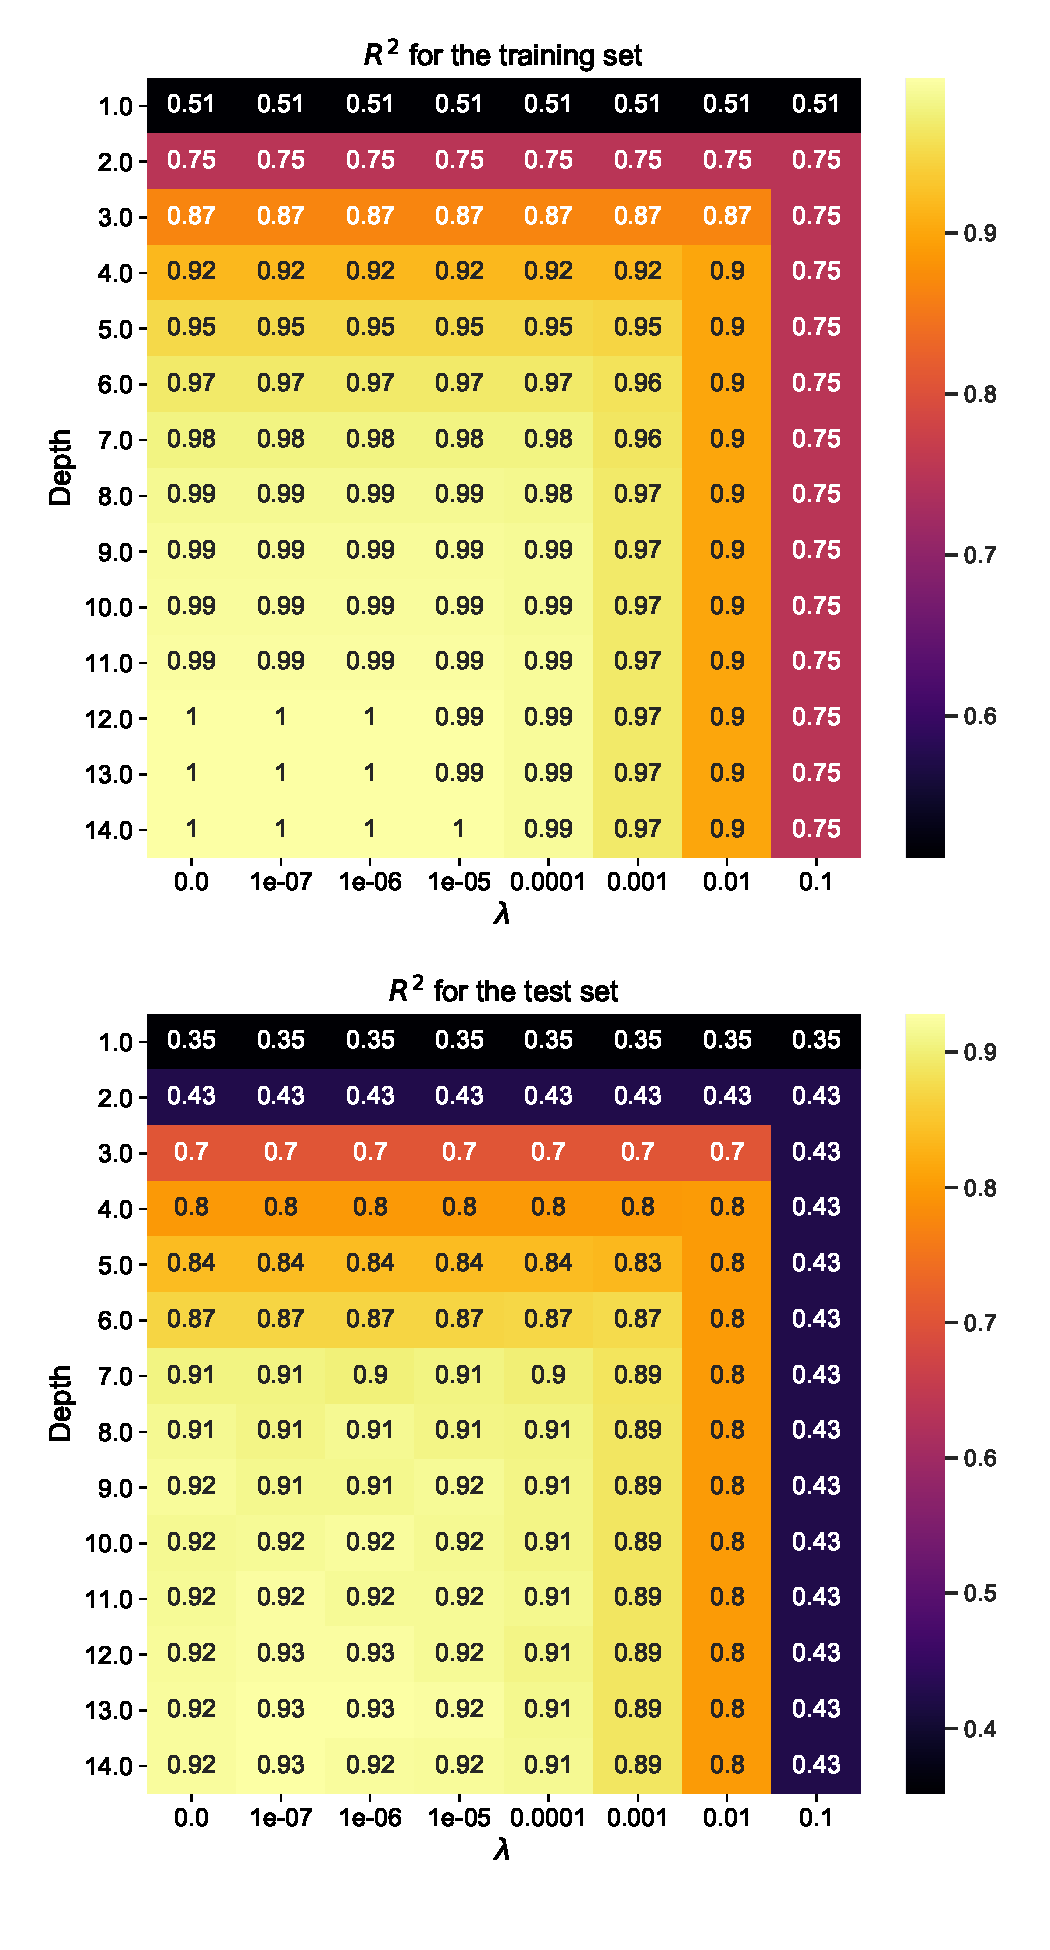
\includegraphics[width=.49\textwidth]{Figures/DecisionTree_R2.pdf}
    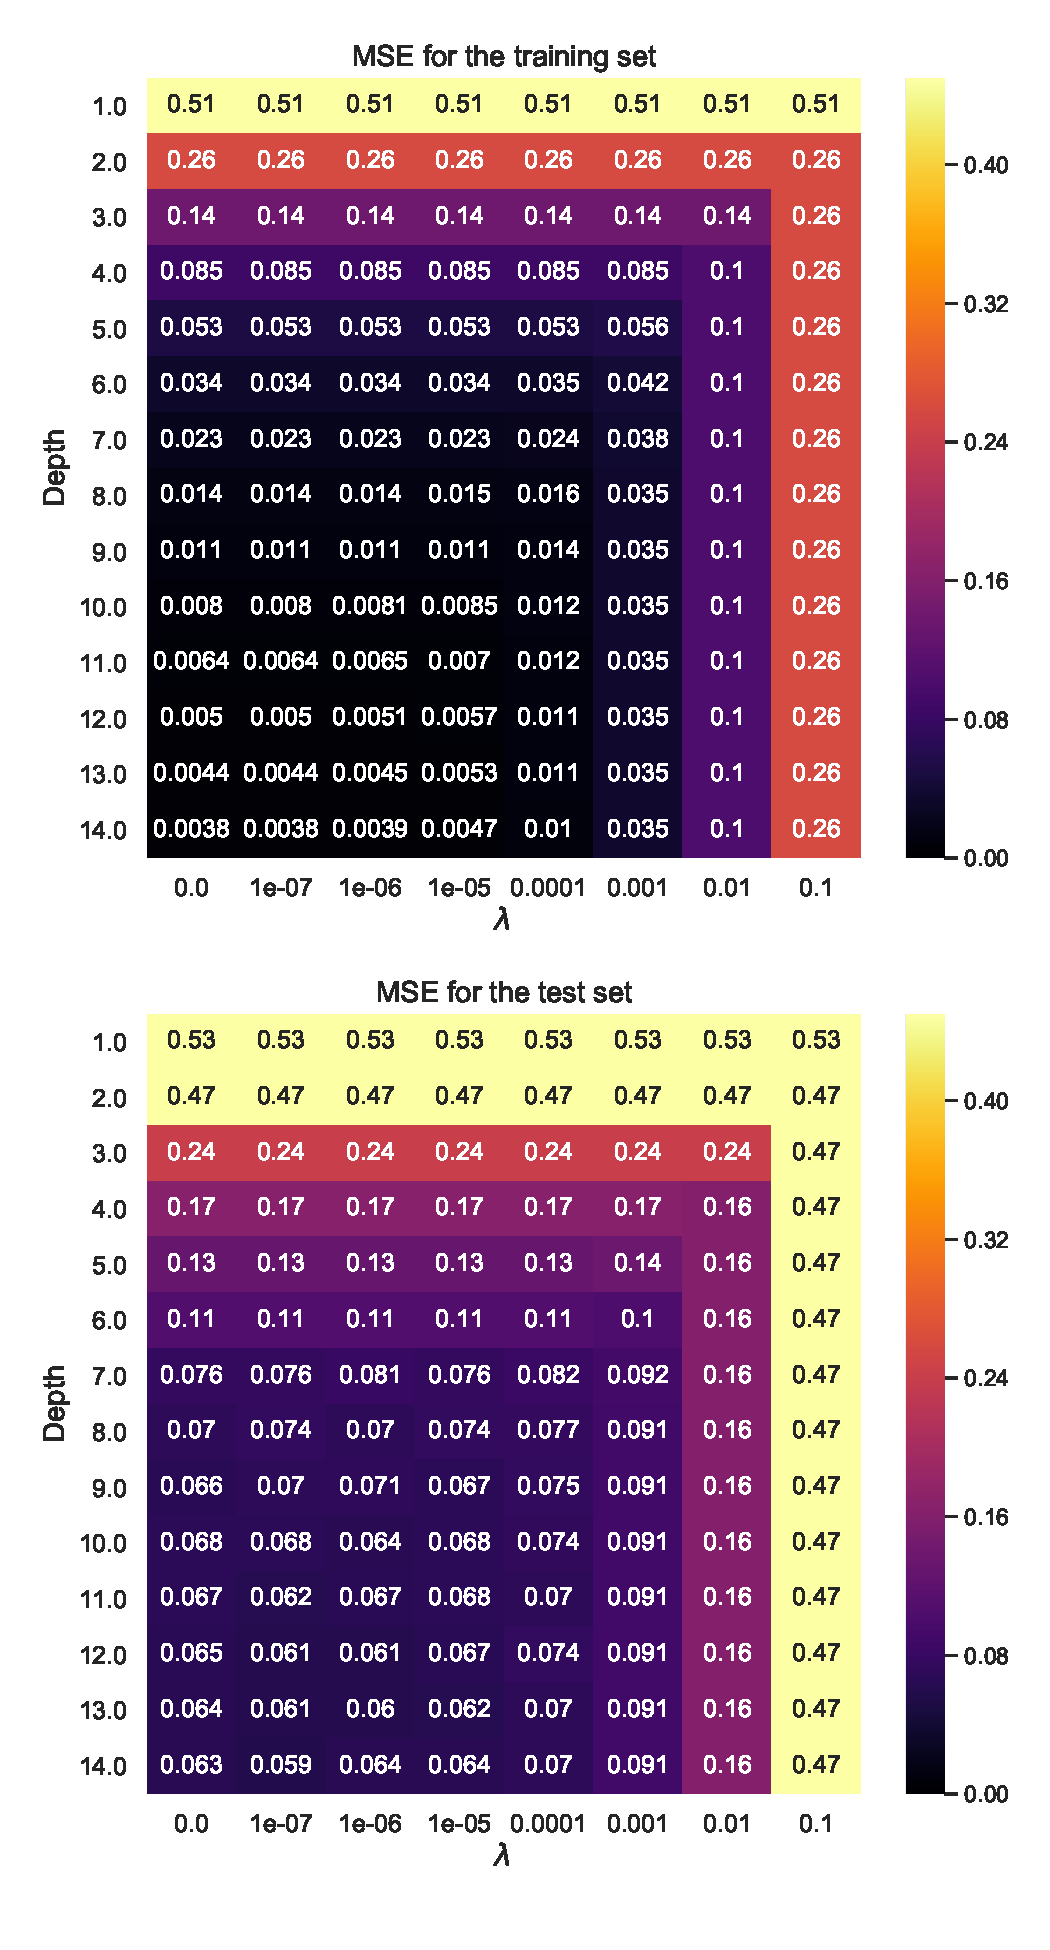
\includegraphics[width=.49\textwidth]{Figures/DecisionTree_MSE.pdf}
    \caption{Test and training MSE and $R^2$ scores for the decision tree method as functions of depth and pruning parameter $\lambda$.}
    \label{fig: Decision Tree scores}
\end{figure}

\begin{figure}[!ht]
    \centering
    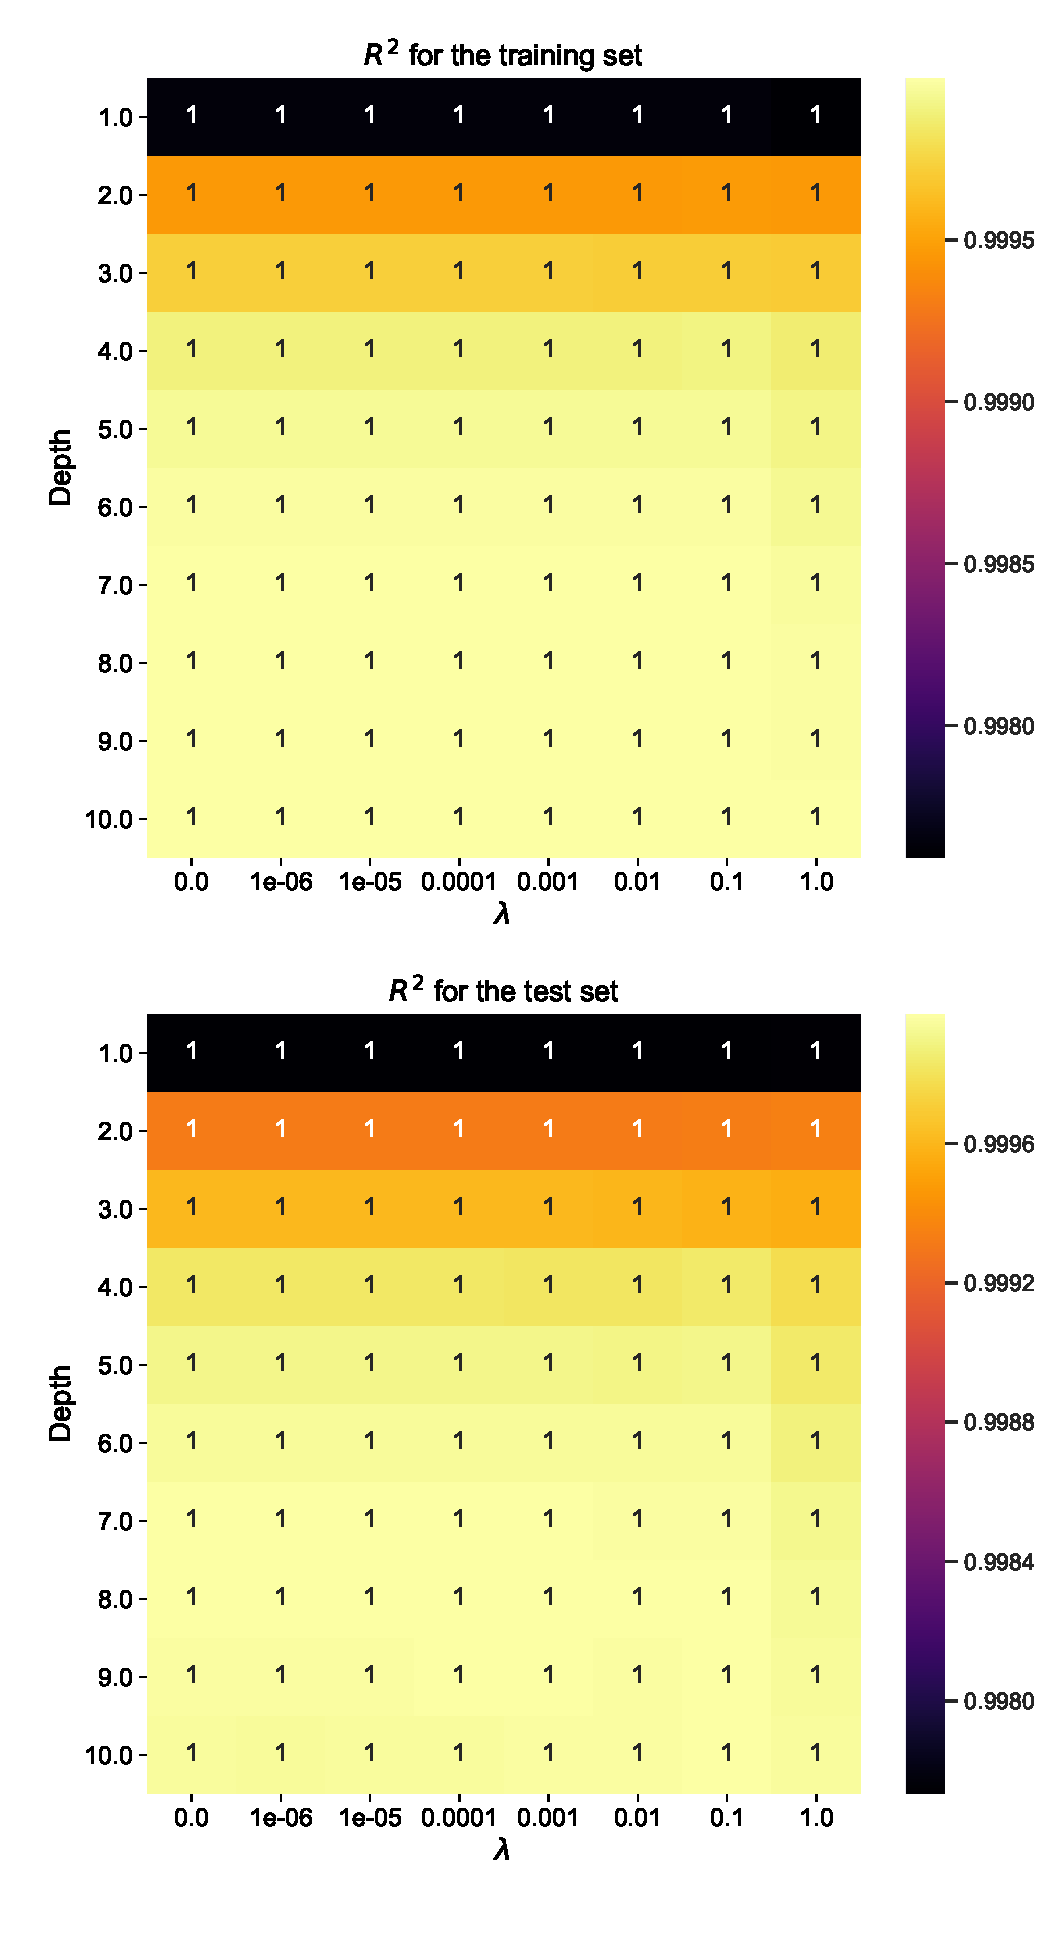
\includegraphics[width=.49\textwidth]{Figures/XGB_R2.pdf}
    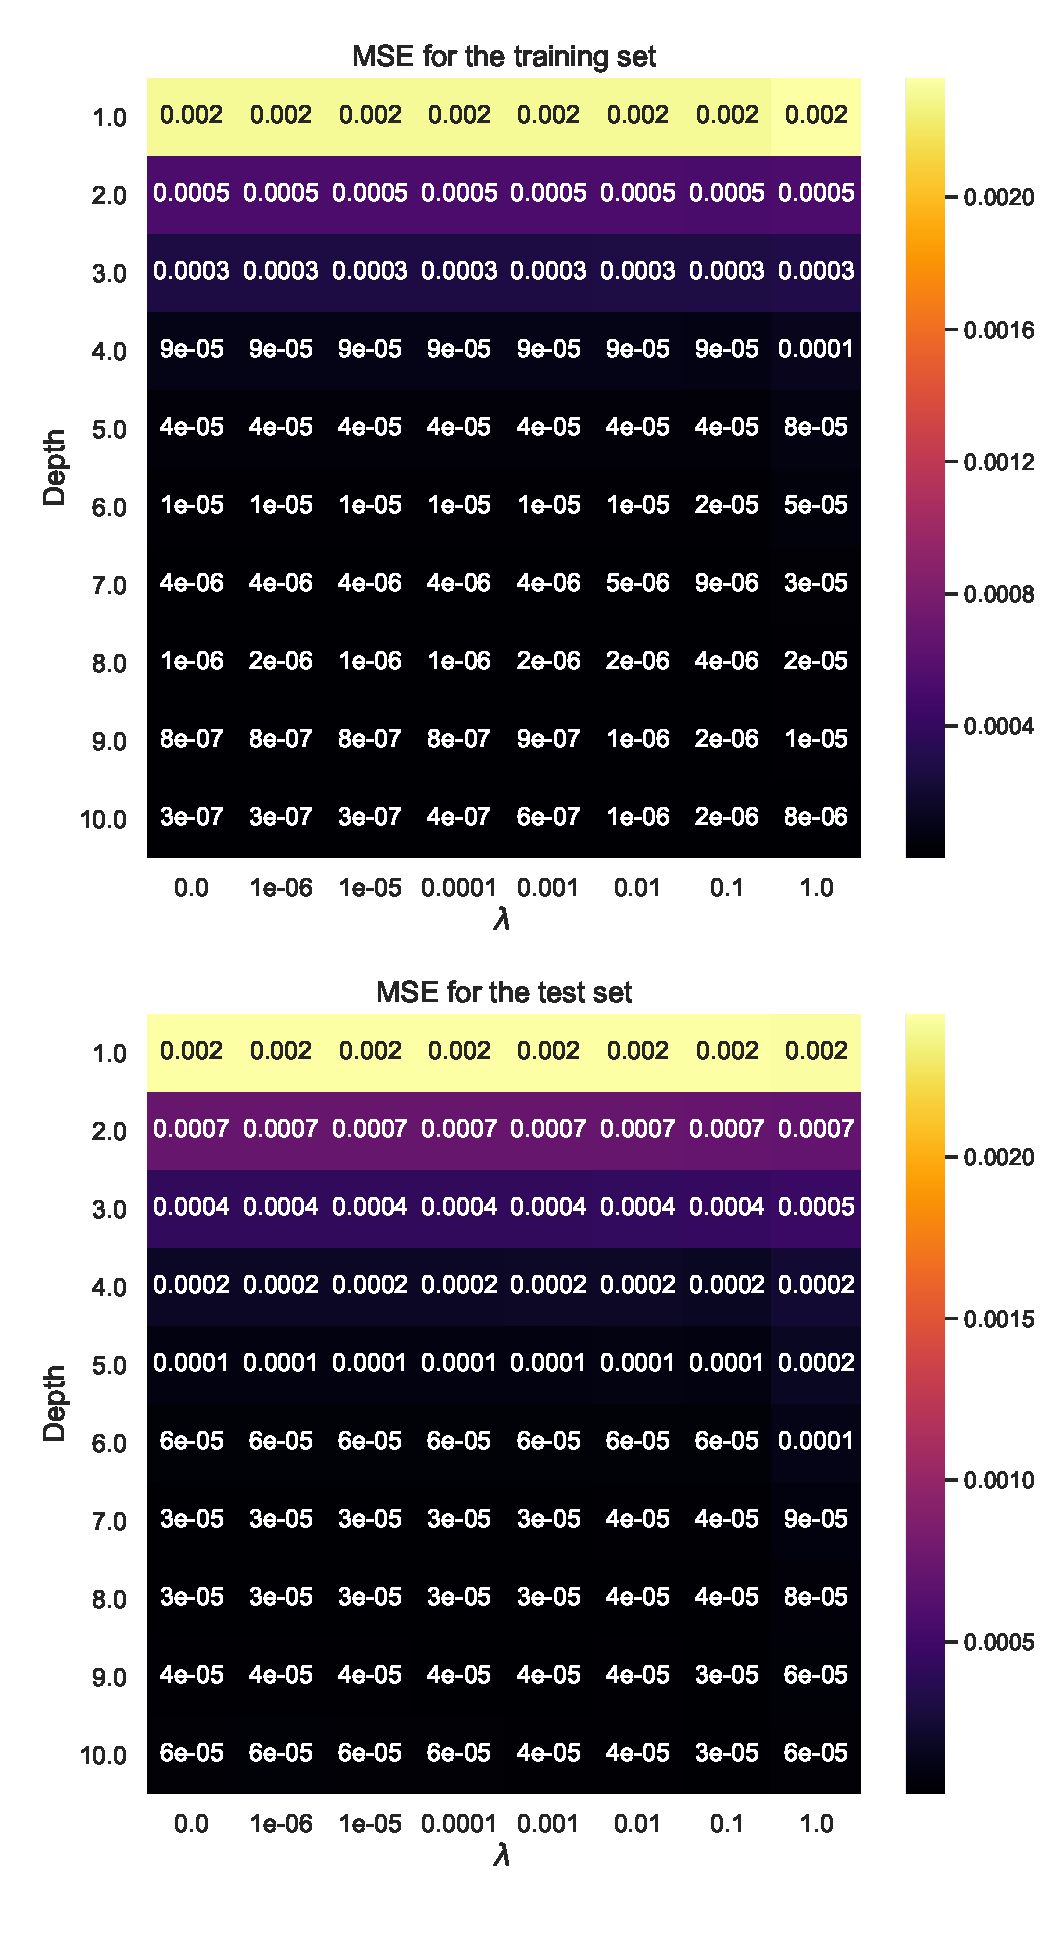
\includegraphics[width=.49\textwidth]{Figures/XGB_MSE.pdf}
    \caption{Test and training MSE and $R^2$ scores for the XGBoost method, acquired with learning rate $\eta \approx 0.0776$, as functions of depth and $\lambda$. $\lambda = 10^{-6}$, depth $= 8$ score proved to be the best for this learning rate.}
    \label{fig: XGBoost scores}
\end{figure}



\end{document}

